\chapter{Multitable Methods and Microbiome Data Integration}
\label{ch:multitable}

The simultaneous study of multiple measurement types is a frequently encountered
problem in practical data analysis. It is especially common in microbiome
research, where several sources of data -- for example, 16S, metagenomic,
metabolomic, or transcriptomic data -- can be collected on the same physical
samples \citep{Franzosa2015, McHardy2013}. There has been a proliferation of
proposals for analyzing such multitable microbiome data, as is often the case
when new data sources become more readily available, facilitating inquiry into
new types of scientific questions \citep{Fukuyama2017, Rahnavard2017,
  Chaudhary2017, Chalise2017}.

However, stepping back from the rush for new methods for multitable analysis in
the microbiome literature, it is worthwhile to recognize the broader landscape
of multitable methods, as they have been relevant in problem domains ranging
from economics \citep{hannan1967canonical} to robotics
\citep{vlassis2000supervised} to genomics \citep{gomez2014data}. In different
contexts, these techniques are called data integration, multi-omic, and
multitask methods, for example. Of course, there is no unique optimal algorithm
to use across domains -- different instances of the multitable problem possess
specific structure or variation that are worth incorporating in methodology.

Our purpose here is not to develop new algorithms, but rather to (1) distill the
relevant themes across different analysis approaches and (2) provide concrete
workflows for approaching analysis, as a function of ultimate analysis goals and
data characteristics (heterogeneity, dimensionality, sparsity, ...).
Towards the second goal, we have made code for all analysis and figures
available online at
\url{https://github.com/krisrs1128/well\_microbiome\_expers}.

First, though, why does anyone bother collecting multiple sources of data, and
why can't these sources simply be combined into a single, unified table for
subsequent analysis? One answer is that many scientific problems can only be
answered by collecting several complementary measurement types. Indeed, the
situation is analogous to using many types of sensors to study a single system
from many perspectives. Further, while in certain supervised problems, it is
enough to predict a single measurement of interest, with other sources primarily
collected to provide better features, there are often an additional relational
components to the analysis: how do different types of measurements covary with
one another? Here, it is of interest to provide a representation of
the data that facilitates comparisons across tables, rather than just comparing
each table with a single response of interest. This richer scientific question
motivates the development of methods distinct from those used to analyze a
single measurement type at a time.

For more concrete motivation, we consider data from the WELL-China study, which
is focused on the relationships between various indicators of wellness
\citep{wellchina}. In this study, 1969 individuals\footnote{Though sampling is
  still ongoing.} underwent clinical examinations, filled out wellness surveys
(covering topics such as exercise, sleep, diet, and mental health, for example),
and provided stool samples, used for 16S sequencing and metabolomic analysis. To
date, 16S sequencing data is available for 221 of these participants. Evidently,
various interesting relational questions can be investigated using this data
source.

For the purpose of illustration, we focus on one relatively narrow question that
can be addressed using this data: How is the distribution of lean and fat mass
across the body related to patterns of microbial abundance? The measurement
types most relevant in this analysis are DEXA scans and 16S sequencing abundances.
DEXA scans use relative X-ray absorption to gauge the amount of lean and fat body
mass within a region of the body being scanned. We have access to these
lean and fat body mass measurements at several body sites -- arms, legs, trunk,
etc. -- along with related body type variables, like height, age, and android
and gynoid fat measurements. In total, there are 36 of these variables. 16S
sequencing is a technology for gauging the abundance of different bacterial
species in the gut by counting the alignments of reads to the 16S gene, a
component of all bacterial genomes with enough variation to allow discimination
between different individual species. We have counts associated with 2565
species across 181 genera, though the vast majority are present in low
abundances.

This question of the relationship between lean and fat mass distribution
(informally, ``body type'') and the microbiome is motivated by findings that
certain taxonomic groups are over or underrepresented as a function of an
individual's Body Mass Index (BMI) \citep{ley2006microbial, turnbaugh2009core,
  ley2005obesity, ley2010obesity}. Further, since the distribution of fat is
often more related to underlying biological mechanisms than overall body mass
\citep{matsuzawa2008role}, and since this distribution is mediated by specific
metabolic pathways, there is reason to suspect that a joint analysis of DEXA and
16S microbial abundance data might yield a more complete view of the
relationship between the microbiome and body type.

\section{Classical multivariate methods}

Methods from classical multivariate statistics are a mainstay of single-table
microbiome data analysis, so it is natural to revisit them before surveying
extensions to the multitable setting. Here we explore a few of the classically
studied multitable methods that fit nicely into the modern microbiome data
analysis toolbox. We first describe a naive approach based on Principal
Components Analysis (PCA) -- naive because it lifts a single-table method to the
multiple table setting without any special considerations -- before studying
approaches that directly characterize covariation across several tables:
Canonical Correlation Analysis (CCA), Multiple Factor Analysis (MFA), and
Principal Component Analysis with Instrumental Variables (PCA-IV).

The earliest multitable method (CCA) was published in 1936, where the motivating
data analysis problem was to relate prices of groups of commodities
\citep{hotelling1936relations}. There are two notable aspects of data analysis
in this classical paradigm which no longer hold in modern statistics,
\begin{itemize}
  \item Even when many samples could be collected, there were typically
    only a few features for each samples, and it was straightforwards to study
    all of them simultaneously. It is now possible to automatically collect a
    large number of features for each observation.
  \item Before electronic computers had been invented, it was important that all
    statistical quantities be easy to calculate, typically necessitating
    analytical formulas for parameter estimates. This is no longer an important
    limitation due to modern computation.
\end{itemize}

These changes have driven the development of high-dimensional methods and
facilitated the adoption of iterative, more computationally-intensive
approaches.

Nonetheless, it is worth reviewing these original approaches, both to understand
the context for many modern techniques, as well as to have an easy starting
point for practical data analysis. Indeed, these more established methods tend
to be the most readily available through statistical computing packages and can
provide a benchmark with which to compare more elaborate, modern methods.

\subsection{PCA}
\label{subsec:pca}

The simplest approach to dealing with multiple tables is to combine them into
one and apply a single-table method, for example, PCA. That is, write
\begin{align*}
X = \left[X^{(1)} \vert \dots \vert X^{(L)}\right] \in \reals^{n \times p},
\end{align*}
where $p = \sum_{l = 1}^{L}p_{l}$, and compute the SVD $X = UDV^{T}$. The
$K$-principal component directions are the first $K$ columns $v_{1}, \dots,
v_{K}$, while the associated scores are reweighted rows $d_{1}u_{1}, \dots,
d_{K}u_{K}$. We call this method concatenated PCA.

While this does not account for the multitable structure of the data, it does
accomplish two goals,
\begin{itemize}
\item Through the principal component scores, it provides a visualization of the
  relationships between samples, based on all features.
\item Through the principal component directions, it gives a way of relating
  features within and across the multiple tables.
\end{itemize}

However, two drawbacks of this approach are worth noting,
\begin{itemize}
  \item It does not provide a summary of the relationship between the sets of
    variables defining the tables -- it can only relate pairs of variables.
  \item If some tables have many more variables than others, they can dominate
    the resulting ordination.
\end{itemize}

These limitations are addressed by CCA and MFA, discussed in Sections
\ref{subsec:cca} and \ref{subsec:mfa}, respectively.

We provide one geometric and one statistical motivation for PCA. The geometric
motivation is that, if each row $x_{i}$ of $X$ is viewed as a point in
$p$-dimensional space, then the principal component directions provide the best
$K$-dimensional approximation to the data, see Figure \ref{fig:pca-approx}.
Formally, recall that $VV^{T}x_{i}$ is the projection of $x_{i}$ onto the
subspace spanned by the columns of $V$. PCA identifies the orthogonal matrix $V
\in \reals^{p \times K}$ such that
\begin{align*}
\sum_{i = 1}^{n}\|x_{i} - VV^{T} x_{i}\|_{2}^{2}
\end{align*}
is minimized. The principal component scores are then the coordinates of the
projected points with respect to this subspace.

\begin{figure}
  \centering
  \includegraphics[width=0.5\textwidth]{figure/multitable/pca/proj_plot_1}
  \caption{A geometric motivation for PCA. The first principal component spans
    the one-dimensional subspace $V$ minimizing the squared error between points
    and their projections, $\sum_{i = 1}^{n}\|\left(I -
    VV^{T}\right)x_{i}\|_{2}^{2}$. The black points represent the scaled values
    for two of the body composition variables -- weight and total fat mass --
    while the purple points are the projections onto the first principal
    component. Contrast this with Figures \ref{fig:pca-approx-2} and
    \ref{fig:pca-approx-3}, where variables other than and fat mass are taken
    into account.}
  \label{fig:pca-approx}
\end{figure}

\begin{figure}
  \centering
  \includegraphics[width=0.5\textwidth]{figure/multitable/pca/var_plot}
  \caption{A statistical motivation for PCA. Each histogram is computed from the
    linear combinations $\left(c^{j^{T}}x_{i}\right)$, for $c^{j}$ equal to the
    first and second principal components, the vector $\frac{1}{n}\mathbf{1}$,
    and a normalized random multivariate Gaussian. At least among these four
    vectors, the scores obtained from the first PC have the largest variance. It
    is a theorem that its variance is in fact maximal among all linear
    combinations with unit-length vectors.}
  \label{fig:pca-var}
\end{figure}

The second interpretation is that PCA finds a low-dimensional representation of
the $x_{i}$ such that the resulting points have maximal variance. Qualitatively,
this is a desirable property, because it means that the simpler representation
preserves most of the variation present in the original data, see Figure
\ref{fig:pca-var}. In this figure, histograms of the scores associated with four
linear combinations of the original body composition measurements are displayed
side by side, to emphasize the fact that the linear combination $x^{T}v_{1}$
associated with the first principal component $v_{1}$ has the largest variance
among a few natural choices.

Formally, suppose that the $x_{i}\in\reals^{p}$ are drawn independently from
some distribution $\P$, so that the variance is $\Covsubarg{\P}{x_{i}} =
\Sigma$. Consider an arbitrary linear combination of $x_{i}$'s $p$ coordinates:
$z_{i} := c^{T}x_{i}$ for some $c \in \reals^{p}$. The first PCA direction gives
the unit-length $c$ such that the variance of this coordinate,
$\Varsubarg{\P}{z_{i}} = c^{T}\Sigma c$, is maximal. The second direction gives
the linear combination that maximizes variance, subject to being orthogonal to
the first, and so forth.

While our description of the method of concatenating multiple tables into a
single one has focused on PCA, note that other single table methods could be
applied instead. For example, suppose there are multiple data types -- say
count, categorical, and continuous -- across tables. Then, it is possible to
define a new distance between samples as a mixture of distances based on several
tables. For example, Jaccard, $\chi^{2}$, and Euclidean distances can be applied
to binary, count, and real valued tables. The combined distance can then be
input into any distance-based single-table procedure, like multidimensional
scaling or hierarchical clustering. The primary downside of this approach is
that the resulting distance only allows a comparison between samples, but not
across features.

PCA is a very widely used technique, and some standard references include
\citep{friedman2001elements, mardia1980multivariate, pages2014multiple}.
Nonetheless, it is not ideal in the multitable setting.

\subsubsection{Example}
\label{subsubsec:pca_example}

Figure \ref{fig:loadings} and \ref{fig:scores_android_fm} illustrate this
approach on body composition and bacterial abundance data from the WELL-China
study. Note that we have subsetted to only women, since men and women have very
different body compositions, and we have slightly more data for women. Further,
the 16S data have been variance stabilized according the methodology proposed in
\citep{Anders2010} and filtered to only those species that have count $\geq 5$
in at least 7\% of samples.

Figure \ref{fig:loadings} displays the loadings associated with this
concatenated PCA approach, where body composition (36 columns) and 16S
abundances (372 columns) were combined into one dataset (408 columns). Columns
associated with bacterial species are displayed as points, shaded by taxonomic
family, while columns associated with body composition variables are labeled
with text.

Most body composition variables lie on the top right, in a direction
approximately orthogonal to the main direction of variation among species.
Columns that are highly correlated -- e.g., right (R) and left (L) leg fat mass
(FM) -- have loadings nearly equal to one another. Among species, the most
notable pattern is the concentration of Ruminococcaceae on the right.

To identify relationships between species and body composition variables, it
would be of interest to isolate those species with large contributions along the
axis defined by linking the center of the variables and the origin. Relatively
few such species stand out, though note that there is nothing in this
algorithm's objective that would seek covariation across tables directly, so the
fact that such associations seem weak with respect to the top two principal
components does not mean such relationships do not exist.

\begin{figure}
  \centering \includegraphics[width=\textwidth]{figure/multitable/pca/loadings}
  \caption{The loadings obtained by applying PCA to the combined body
    composition and microbial abundance data. Species are points, and are shaded
    in by taxonomic family. Body composition variables are plotted as text. The
    size of points and words measures the contribution of the third PC
    dimension. \label{fig:loadings} }
\end{figure}

We can study individual samples with respect to these loadings, by plotting
their projections onto the top two principal components. This is the content of
Figures \ref{fig:scores_android_fm} and \ref{fig:scores_rl_ratio}. These figures
display samples in the same positions, but shaded by android (i.e., abdominal)
fat mass and the difference between variance-stabilized Bacteroidaceae and
Ruminococcaceae\footnote{We pass the difference through $\tanh$ to squash very
  large differences.} counts, respectively. This shading confirms the
observations from the loadings directly using observed data. Indeed, the
increasing android fat mass among samples in the top of Figure
\ref{fig:scores_android_fm} exactly corresponds to the fact that related
variables lie at the top in Figure \ref{fig:loadings}. The largest
Bacteroidaceae vs. Ruminococcaceae differentiation is visible in Figure
\ref{fig:scores_rl_ratio}, which is consistent with the loadings.

In this approach, the loadings provide a description of the relationship between
variables across datasets. Further, scores summarize variation in samples across
multiple datasets. Hence, this heuristic is a natural first step in analyzing
multiple table data. However, considering the difficulty in directly
interpreting the covariation across datasets, as well as the method's failure to
use any sense of covariation in the dimensionality reductions strategy, suggests
that this method should not be the last step of an analysis workflow.
Nevertheless, we now have a baseline with which to compare the more elaborate
methods of subsequent sections.

\begin{figure}
  \centering
  \includegraphics[width=\textwidth]{figure/multitable/pca/scores_android_fm}
  \caption{The scores resulting from PCA applied to the combined body
    composition and microbial abundance data. The first two principal components
    explain about 4\% of the variance. Points are species, shaded in by
    taxonomic family. Text are columns from the body composition data. Points
    and text with small angle between one another are more correlated.
    \label{fig:scores_android_fm} }
\end{figure}

\begin{figure}
  \centering
  \includegraphics[width=\textwidth]{figure/multitable/pca/scores_rl_ratio}
  \caption{The same scores as Figure \ref{fig:scores_android_fm}, but shaded now
    by the transformed ratio of Bacteroidaceae over Ruminococcaceae abundances.
    The slight increase in Ruminococcaceae from left to right is consistent with
    the loadings observed in Figure
    \ref{fig:loadings}.\label{fig:scores_rl_ratio} }
\end{figure}

\subsection{CCA}
\label{subsec:cca}

CCA is a close relative of PCA, designed to compare sets of features across
tables. Like PCA, it provides low-dimensional representations of observations,
but it also allows comparisons at the table level. Suppose for now that there
are only two tables of interest, $X \in \reals^{n \times p_{1}}$ and $Y \in
\reals^{n \times p_{2}}$. Let $\hat{\Sigma}_{XX}, \hat{\Sigma}_{YY}$, and
$\hat{\Sigma}_{XY}$ be the associated covariance estimates. Take the SVD,
$\hat{\Sigma}_{XX}^{-\frac{1}{2}}\hat{\Sigma}_{XY}\hat{\Sigma}_{YY}^{-\frac{1}{2}}
= \tilde{U}D\tilde{V}^{T}$. The canonical correlation directions associated with
the two tables are $u_{k} = \Sigma_{XX}^{-\frac{1}{2}}\tilde{u}_{k} \in
\reals^{p_{1}}$ and $v_{k} = \Sigma_{YY}^{-\frac{1}{2}}\tilde{v}_{k} \in
\reals^{p_{2}}$. These directions give two sets of low-dimensional
representations for each sample, one for each table: $z_{k}^{(1)} = Xu_{k} \in
\reals^{n}$ and $z_{k}^{(2)} = Yv_{k} \in \reals^{n}$. If the two tables are
closely related, then the $z_{k}^{(1)}$ and $z_{k}^{(2)}$ will be very
correlated. The singular values $d_{k}$ are called the canonical correlation
coefficients. Like the eigenvalues in PCA, they characterize the amount of
covariation across tables that can be captured by each additional pair of
directions.

As with PCA, there are many ways to view this procedure -- here we discuss
geometric, statistical, and probabilistic interpretations. Unlike the geometric
interpretation of PCA, the geometric interpretation for CCA identifies point
locations with features, not samples. Specifically, the columns of $X$ and $Y$
are thought of as points in $\reals^{n}$. Consider two subspaces spanning the
columns of $X$ and $Y$, respectively. These subspaces correspond to the linear
combinations of features within each table. Place two ellipses on the respective
subspaces, centered at the origin and with size and shape depending on the
within table covariances $\hat{\Sigma}_{XX}$ and $\hat{\Sigma}_{YY}$. The first
canonical correlation directions are the pair of points, one lying on each
ellipse, such that the angle from the origin to those two points is smallest. In
this sense, it finds a pair of variance-constrained linear combinations of
features within the two tables such that the two combinations appear ``close''
to one another. The second pair of canonical correlation directions identify a
pair of points with a similar interpretation, except they are required to be
orthogonal to the first pair, with respect to the inner product induced by the
covariances in each table.

For a statistical interpretation, the idea of CCA is to find the low-dimensional
representations of the two tables with maximal covariance -- this is analogous
to the maximum variance interpretation. Formally, rows of the two tables are
imagined to be i.i.d. draws from $\P^{XY}$, which has marginals $\P^{X}$ and
$\P^{Y}$. Consider arbitrary linear combinations $z_{i}^{(1)}\left(u\right) =
u^{T} x_{i}$ and $z_{i}^{(2)}\left(v\right) = v^{T}y_{i}$ of samples from the
two tables. The first pair of CCA directions $u_{1}^{\ast}$ and $v_{1}^{\ast}$
are chosen to optimize
\begin{align}
  \maximize_{u \in \reals^{p_{1}}, v \in \reals^{p_{2}}}\medspace
  &\Covsubarg{\P^{XY}}{z_{i}^{(1)}\left(u\right),
    z_{i}^{(2)}\left(v\right)} \label{eq:cancor_optim} \\ \text{subject to }
  &\Varsubarg{\P^{X}}{z_{i}^{(1)}\left(u\right)} = 1 \nonumber
  \\ &\Varsubarg{\P^{Y}}{z_{i}^{(2)}\left(v\right)} = 1. \nonumber
\end{align}
To produce subsequent directions, the same optimization is performed, but with
the additional constraint that the directions must be orthogonal to all the
previous directions identified for that table. Of course, in actual
applications, we estimate these covariances and variances empirically.

This perspective makes it easy to derive the algorithm given at the start of
this section. The empirical version of the optimization problem
\ref{eq:cancor_optim} is
\begin{align}
  \maximize_{u \in \reals^{p_{1}}, v \in \reals^{p_{2}}}\medspace
  &u^{T}\hat{\Sigma}_{XY}v \label{eq:cancor_optim_emp}\\ \text{subject to } &
  u^{T}\hat{\Sigma}_{XX}u = 1 \nonumber \\ & v^{T}\hat{\Sigma}_{YY}v = 1.
  \nonumber
\end{align}

Consider the transformed data, $\tilde{u} = \hat{\Sigma}_{XX}^{\frac{1}{2}}u$
and $\tilde{v} = \hat{\Sigma}_{YY}^{\frac{1}{2}}v$. The
optimization \label{eq:cancor_emp} can now be expressed as
\begin{align}
  \maximize_{\tilde{u} \in \reals^{p_{1}}, \tilde{v} \in
    \reals^{p_{2}}}\medspace
  &\tilde{u}^{T}\hat{\Sigma}_{XX}^{-\frac{1}{2}}\hat{\Sigma}_{XY}\hat{\Sigma}_{YY}^{-\frac{1}{2}}\tilde{v} \label{eq:cancor_trans}
  \\ \text{such that } & \|\tilde{u}\|^{2}_{2} = 1 \nonumber
  \\ &\|\tilde{v}\|_{2}^{2} = 1. \nonumber
\end{align}
The optimal $\tilde{u}_1$ and $\tilde{v}_1$ for this problem are well known --
they're exactly the first left and right eigenvectors of
$\hat{\Sigma}_{XX}^{-\frac{1}{2}}\hat{\Sigma}_{XY}\hat{\Sigma}_{YY}^{-\frac{1}{2}}
= \tilde{U}D\tilde{V}^{T}$, respectively. The argument is standard\footnote{See
  \citep{mardia1980multivariate}, for example.}, but we include it for
completeness.

Let $\xi$ and $\nu$ be potential maximizers of length one. We can find $w_{u}$
and $w_{v}$ such that $\xi = \tilde{U}w_{u}, \nu = \tilde{V}w_{v}$, since
$\tilde{U}$ and $\tilde{V}$ are both orthonormal bases. Since they are length
one, $1 = \|\xi\|^{2}_{2} = w_{u}^{T}\tilde{U}^{T}\tilde{U}w_{u} =
\|w_{u}\|_{2}^{2}$ and similarly $\|w_{v}\|_{2}^{2} = 1$. The objective
\ref{eq:cancor_trans} can be bounded by
\begin{align*}
\xi^{T}\hat{\Sigma}_{XX}^{-\frac{1}{2}}\hat{\Sigma}_{XY}\hat{\Sigma}_{YY}^{-\frac{1}{2}}\nu
&= w_{u}^{T}\tilde{U}^{T}\tilde{U}D\tilde{V}^{T}\tilde{V}w_{v} \\ &=
w_{u}^{T}Dw_{v} \\ &= \sum_{k = 1}^{p_{1} \wedge p_{2}} d_{k}w_{uk}w_{vk}
\\ &\leq d_{1} \sum_{k = 1}^{p_{1} \wedge p_{2}} w_{uk}w_{vk} \\ &\leq d_{1}
\|w_{u}\|\|w_{v}\| = d_{1},
\end{align*}
and this maximum is attained when $w_{u}$ and $w_{v}$ both put all their on the
first coordinate, that is $\xi = \tilde{u}_{1}$ and $\nu = \tilde{v}_{1}$. For
subsequent directions, we repeat the argument but require that $w_{u}$ and
$w_{v}$ have zero on the first columns of $\tilde{U}$ and $\tilde{V}$.

To recover the solutions to the original problem, we reverse the original
variable transformation, yielding optimal $u_{1} =
\Sigma_{XX}^{-\frac{1}{2}}\tilde{u}_{1}$ and $v_{1} =
\Sigma_{YY}^{-\frac{1}{2}}\tilde{v}_{1}$.

A probabilistic interpretation of this procedure views it as estimating the
factors in an implicit latent variable model. In particular,
\citep{bach2005probabilistic} supposes that $x_{i}$ and $y_{i}$ are drawn i.i.d.
from the model,
\begin{align*}
  \xi_{i} := \left(\xi_{i}^{s}, \xi_{i}^{x}, \xi_{i}^{y}\right) &\sim
  \Gsn\left(0, I_{d}\right) \\ x_{i} \vert \xi_{i} &\sim \Gsn\left(\mu_{x} +
  W_{X}\xi_{i}^{s} + B_{X}\xi_{i}^{x}, I_{d} \right) \\ y_{i} \vert \xi_{i}
  &\sim \Gsn\left(\mu_{Y} + W_{Y}\xi_{i}^{s} + B_{Y}\xi_{i}^{y}, I_{d}\right)
\end{align*}
That is, each sample is associated with a $d$-dimensional latent variable
$\xi_{i}$, drawn from a spherical normal prior. A few of the coordinates of
these latent variables, $\xi_{i}^{s}$, contribute to shared structure, through
$W_{X}$ and $W_{Y}$. The remaining coordinates model table-specific structure,
through $B_{X}$ and $B_{Y}$. It can be shown that the posterior expectations of
the latent $\xi_{i}^{s}$ (assumed $\in \reals^{K}$) given the observed tables
must lie on the subspace defined by the CCA directions. More precisely,
\begin{align*}
  \Earg{\xi_{i} \mid x_{i}^{(1)}} \in \text{span}\left(z_{1}^{(1)}, \dots,
  z_{K}^{(1)}\right),
\end{align*}
and
\begin{align*}
  \Earg{\xi_{i} \mid x_{i}^{(2)}} \in \text{span}\left(z_{1}^{(2)}, \dots,
  z_{K}^{(2)}\right).
\end{align*}

Finally, we observe that the logic for CCA generalizes to an arbitrary number
$L$ of tables, by summing all pairwise covariances. That is, the instead of
finding directions $c_{k}^{(1)}$ and $c_{k}^{(2)}$ maximizing
$\Covsubarg{\P^{(1)}, \P^{(2)}}{c_{k}^{(1)T}x_{i}^{(1)},
  c_{k}^{(2)T}x_{i}^{(2)}}$ subject to normalization and orthogonality
constraints, we can seek directions $c_{k}^{(1)}, \dots, c_{k}^{(L)}$ that
maximize the sum of cross-covariances $\sum_{l,l^{\prime} = 1}^{L}
\Covsubarg{\P^{(l)}, \P^{(l^{\prime})}}{c_{k}^{(l) T}x_{i}^{(l)},
  c_{k}^{(l^{\prime})}x_{i}^{(l^{\prime})}}$.

\subsubsection{Example}
\label{subsubsec:cca_example}

We next apply CCA to the WELL-China body composition and microbiome data, with
particular interest in how the results compare with those of Section
\ref{subsubsec:pca_example}. To this end, we provide analogous loadings and
scores plots in Figures \ref{fig:cca_loadings} through
\ref{fig:cca_scores_rl_ratio}. However, note that the data are \textit{not}
quite the same between the two analysis -- we have filtered down to species
passing a filter, which reduces the number of species to 66, from 2565. This
very aggressive filtering is necessary because CCA requires estimation of
covariances matrices $\Sigma_{XX}, \Sigma_{XY}$, and $\Sigma_{YY}$, which is
impossible for $p > n$ and highly unstable when $p$ is a large fraction of $n$.
Besides this stronger filtering, all preprocessing steps remain the same as in
Section \ref{subsubsec:pca_example}.

\begin{figure}
  \centering \includegraphics[width=\textwidth]{figure/multitable/CCA/loadings}
  \caption{The CCA analog of the PCA loadings plot in Figure \ref{fig:loadings}.
    loadings obtained by applying CCA to the combined body composition and
    microbial abundance data. Each point is a species, and text are body
    composition variables. Species are shaded in according to taxonomic family,
    and the size of points corresponds to the third CCA dimension. Text and
    point that are close to one another have similar patterns of abundance
    across samples.
      \label{fig:cca_loadings} }
\end{figure}

Figure \ref{fig:cca_loadings} provides the analog of CCA loadings. To be
precise, let $X \in \reals^{102\times 36}$ be the matrix of body composition
measurements and $Y \in \reals^{102 \times 66}$ be the variance-stabilized
microbial abundances. As before, write $u_{k} \in \reals^{36}, v_{k} \in
\reals^{66}$ for the $k^{th}$ canonical correlation directions. Then, Figure
\ref{fig:cca_loadings} displays text labels for column $j$ of the body
composition variables at location $\left(u_{j1}, u_{j2}\right)_{j = 1}^{36}$ and
shaded points for the $j^{th}$ species at position $\left(v_{j1},
v_{j2}\right)_{j = 1}^{66}$.

As in the concatenated PCA, we find that the groups of variables occupy
separates spaces. Our interpretation is that sequences further to the left are
correlated with the body variables further to the left, which are all in some
way variants of body mass. Note that age is negatively correlated with total fat
mass, which is why it appears on the opposite end. Among the abundant species
that remain, there is limited clustering according to taxonomic group, though
the Bacteroideceae and Ruminoccocus do appear restricted to the bottom and top
right, respectively.

In Figure \ref{fig:cca_scores_linked} we plot the corresponding scores. Note
that in CCA, there are two sets of scores for each $k$, the $Xu_{k}$ and
$Yv_{k}$. Indeed, the CCA objective finds directions that maximizes the
correlation between these scores. This figure displays both sets of scores,
colored differently according to the table to which they are associated. The
pairs of scores for each individual sample are drawn with small links. Since
most links are relatively short, linear combinations of the two tables could be
found that optimized the objective -- indeed, the top two canonical correlations
are 0.968 and 0.957. However, some caution is necessary here, and a more honest
evaluation would be based on scores obtained by projecting new samples onto the
original CCA directions. This is especially important in this nearly
high-dimensional setting, where covariance estimation may be unreliable.

Aside from the fact that samples appear as pairs, interpretation proceeds as in
a PCA scores plot, as in Figure \ref{fig:scores_android_fm}. For example,
Figures \ref{fig:cca_scores_android_fm} and \ref{fig:cca_scores_rl_ratio}
display the samples shaded in by android fat mass and Bacteroidaceae vs.
Ruminococcaceae difference, respectively, as in Figures
\ref{fig:scores_android_fm} and \ref{fig:cca_scores_rl_ratio}. The association
between these variables and the sample positions is not as strong as when
performing PCA on the combined table. This is to be expected, however, as PCA
maximizes variance without any thought to covariance, and the body
composition table alone has a large portion of its variance related to android
fat mass.

\begin{figure}
  \centering
  \includegraphics[width=\textwidth]{figure/multitable/cca/scores_linked}
  \caption{The scores resulting from CCA applied to the combined body
    composition and microbial abundance data. Each measurement type provides a
    different set of scores for the observed samples, and the similarity between
    the sets of scores is reflected in the CCA objective. Each sample appears as
    two separate circles, since there is one score per measurement type. A light
    line links the two appearances of each sample. Colors distinguish the two
    table sources. The higher the CCA objective, the shorter the links between
    pairs.
    \label{fig:cca_scores_linked}}
\end{figure}

\begin{figure}
  \centering
  \includegraphics[width=\textwidth]{figure/multitable/cca/scores_android_fm}
  \caption{The scores resulting from CCA applied to the combined body
    composition and microbial abundance data, shaded in by android fat mass. The
    positions of points are identical to those in Figure
    \ref{fig:cca_scores_linked}, and other than the shading, the plots are read
    in the same way. The first two CCA dimensions suggest smooth variation
    across samples, according to amount of android fat
    mass. \label{fig:cca_scores_android_fm} }
\end{figure}

\begin{figure}
  \centering
  \includegraphics[width=\textwidth]{figure/multitable/cca/scores_rl_ratio}
  \caption{The same scores as Figure \ref{fig:cca_scores_android_fm}, but shaded
    now by the difference in Bacteroidaceae to Ruminococcaceae
    abundances. \label{fig:cca_scores_rl_ratio} }
\end{figure}

\subsection{Co-Inertia Analysis}

Co-Inertia Analysis (CoIA) emerged in ecology to facilitate analysis of
variation in species abundance as a function of environmental conditions
\citep{doledec1994co}. It can be viewed as a slight modification of CCA. Again,
we seek sets of orthonormal directions $\left(u_{k}\right)_{k = 1}^{K}$ and
$\left(v_{k}\right)_{k = 1}^{K}$ such that the associated projections $Xu_{k}$
and $Yv_{k}$ explain most of the covariation between the tables. Unlike CCA,
CoIA finds its first directions by maximizing the covariance -- not the
correlation -- between scores,
\begin{align*}
\maximize_{u \in \reals^{p_{1}}, v \in \reals^{p_{2}}}\medspace &u^{T}X^{T}Yv
\\ \text{ such that}\medspace &\|u\| = 1\\ &\|v\| = 1,
\end{align*}
with subsequent directions found by the same optimization, after adding the
constraint that they are orthogonal to the previously derived directions.

The only difference with the objective in equation \ref{eq:cancor_optim_emp} is
that norm constraint is imposed on $u$ and $v$ directly, rather than their
transformations $\Sigma_{XX}^{\frac{1}{2}}u$ and $\Sigma_{YY}^{\frac{1}{2}}v$.
It is in this sense that the CCA objective maximizes the correlation between
scores, while CoIA maximizes the covariance.

The solutions $\left(u_{k}\right)_{k = 1}^{K}$ and $\left(v_{k}\right)_{k =
  1}^{K}$ can be obtained as the first $K$ left and right eigenvectors from the
SVD of $X^{T}Y$, as opposed to the first $K$ generalized eigenvectors, as in
CCA. The proof of this fact is almost identical to the derivation in Section
\ref{subsec:cca}, for CCA.

\subsubsection{Example}
\label{subsubsec:coia_example}

We apply CoIA to the same data as used in Section \ref{subsubsec:cca_example},
as CoIA also needs to estimate the covariance between tables, which is difficult
when the number of species is large. The loadings are displayed in Supplementary
Figure \ref{fig:coia_loadings}, and they are similar to those in Figure
\ref{fig:cca_loadings}. However, the associated scores are quite different than
those found using CCA. Compare Figure \ref{fig:coia_scores_android_fm}, which
shades samples by android fat mass, or Supplemental Figure
\ref{fig:coia_scores_rl_ratio}, which shades them by Bacteroides vs.
Ruminococcaceae differences, with Figures \ref{fig:cca_scores_android_fm} and
\ref{fig:cca_scores_rl_ratio} for CCA. The scores for CoIA are not so closely
aligned across tables, but they exhibit a clearer gradient across supplemental
variables. We find that the scores are not nearly as closely aligned as they are
for CCA (see Figure \ref{fig:cca_scores_android_fm}), but that they are more
strongly associated with variation in android fat mass, as in the concatenated
PCA result of Figure \ref{fig:scores_android_fm}. It is not clear whether this
phenomena -- the CoIA scores being more similar to those from PCA than CCA --
holds in general, or what it is about the change in inner products between CoIA
and CCA that is responsible for this difference.

\begin{figure}
  \centering
  \includegraphics[width=\textwidth]{figure/multitable/coia/scores_android_fm}
  \caption{The normalized scores from each table, displayed simultaneously, as
    obtained by CoIA. This is the analog of Figure
    \ref{fig:cca_scores_android_fm} from CCA, though the aspect ratio has been
    adjusted according to the relative amount of variance explained by the first
    two CoIA axes.
    \label{fig:coia_scores_android_fm} }
\end{figure}

\subsection{MFA}
\label{subsec:mfa}

MFA gives an alternative approach to producing scores and relating features
across multiple tables \citep{pages2014multiple}. It can be understood as a
refined version of the concatenated PCA described in Section \ref{subsec:pca}
that reweights tables in a way that prevents any one table from dominating the
resulting ordination Specifically, MFA is a concatenated PCA on the matrix
\begin{align*}
X := \left[\frac{1}{\lambda_{1}\left(X^{(1)}\right)}X^{(1)} \vert \dots \vert
  \frac{1}{\lambda_{1}\left(X^{(L)}\right)}X^{(L)}\right],
\end{align*}
which reweights each table by its largest eigenvalue. This procedure is the
multitable analog of the common practice of standardizing variables before
performing PCA.

The resulting MFA directions and scores can be interpreted in the same way as
those from PCA -- the MFA directions still specify the relationship between
measured features, and the position of each sample's projection describes the
relative value of each feature for that sample. Moreover, MFA gives a way of
comparing entire tables to each other, called a ``canonical analysis''
\citep{pages2004multiple}. A $K$-dimensional representation of the $l^{th}$
group is given by
\begin{align*}
\left[\mathcal{L}\left(z_{1}, X^{(l)}\right), \dots, \mathcal{L}\left(z_{K},
  X^{(l)}\right)\right]
\end{align*}
where $z_{k} = d_{k}u_{k} \in \reals^{n}$ is the $k^{th}$ column of principal
component scores and
\begin{align*}
  \mathcal{L}\left(z_{k}, X^{(l)}\right) =
  \frac{\lambda_{k}\left(X\right)}{\lambda_{1}\left(X^{(l)}\right)}\tr\left(X^{(l)}X^{(l)
    T} z_{k}z_{k}^{T}\right) =
  \frac{\lambda_{k}\left(X\right)}{\lambda_{1}\left(X^{(l)}\right)}\|X^{(l) T}
  z_{k}\|^{2}_{2}
\end{align*}
is a measure of aggregate similarity between the coordinates in the $l^{th}$
table and the $k^{th}$ column of scores. According to this definition, if the
samples, as represented by the $l^{th}$ table, have high correlation with the
$k^{th}$ dimension of scores, then the canonical analysis displays positions the
$l^{th}$ table far in the $k^{th}$ direction. Plotting these table-level
coordinates helps resolve which tables measure similar underlying variation.

\subsection{PCA-IV}
\label{subsec:pcaiv}

PCA-IV adapts the dimensionality reduction ideas of PCA to the multivariate
regression setting \citep{rao1964use}. It can also be viewed as a version of PCA
that chooses a dimension reduction of $X$ based on its ability to predict $Y$.
In this sense, it anticipates methods like Partial Least Squares, Canonical
Correspondence Analysis, the Curds \& Whey procedure, the Graph-Fused Lasso and
Bayesian multitask learning, which are described in Sections \ref{subsec:PLS},
\ref{subsec:canonical-correspondence}, \ref{subsec:cw},
\ref{subsec:graph_fused_lasso}, and \ref{subsec:bayesian_multitask}
respectively.

Formally, suppose we are predicting $y_{i} \in \reals^{p_{1}}$ from $x_{i} \in
\reals^{p_{2}}$. Since $p_{2}$ may be large, it might be useful to work with a
lower-dimensional representation $z_{i} = V^{T}x_{i} \in \reals^{K}$, that is
potentially more interpretable but still as (or more) predictive of $y_{i}$. As
in PCA, we require that $V$ be orthonormal.

The criterion that PCA-IV uses to identify the loadings $V$ and scores $Z$
mirrors the maximum variance criterion for PCA. Instead of choosing $V$ to
maximize the variance of the $z_{i}$, we choose it to minimize the residual
covariance of $y_{i}$ given $z_{i}$. That is, suppose that $y_{i}$ and $x_{i}$
are jointly normal with mean 0 and covariance
\begin{align*}
\Var_{\P}\begin{pmatrix}y_{i} \\ x_{i}\end{pmatrix} &=
\begin{pmatrix}
  \Sigma_{YY} & \Sigma_{YX} \\ \Sigma_{XY} & \Sigma_{XX}
\end{pmatrix}.
\end{align*}

If $z_{i} = V^{T}x_{i}$, then the joint covariance of $y_{i}$ and $z_{i}$ is
\begin{align*}
  \Var_{\P}\begin{pmatrix} y_{i} \\ z_{i} \end{pmatrix} &=
  \begin{pmatrix}
    \Sigma_{YY} & \Sigma_{YX}V \\ V^{T}\Sigma_{XY} & V^{T}\Sigma_{XX}V
  \end{pmatrix},
\end{align*}
so the residual covariance of $y_i$ given $z_{i}$ is
\begin{align}
  \Sigma_{YY} -
  \Sigma_{YX}V\left(V^{T}\Sigma_{XX}V\right)^{-1}V^{T}\Sigma_{XY}. \label{eq:pca_iv_resid_cov}
\end{align}
\citep{rao1964use} uses the trace to measure the ``size'' of this matrix. The
true population covariances are unknown to us, so we replace them by their
empirical estimates. The formal optimization for PCA-IV then becomes
\begin{align}
  \minimize_{V\in \reals^{p_{2} \times K} \text{ orthonormal}}
  \tr\left(\hat{\Sigma}_{YY} -
  \hat{\Sigma}_{YX}V\left(V^{T}\hat{\Sigma}_{XX}V\right)^{-1}V^{T}\hat{\Sigma}_{XY}\right) \label{eq:pca_iv_obj},
\end{align}
or, equivalently,
\begin{align}
  \maximize_{V\in \reals^{p_{2} \times K} \text{ orthonormal}}
  \tr\left(\hat{\Sigma}_{YX}V\left(V^{T}\hat{\Sigma}_{XX}V\right)^{-1}V^{T}\hat{\Sigma}_{XY}\right) \label{eq:pca_iv_obj_2},
\end{align}

The optimal $V$ are the top $K$ generalized eigenvectors of
$\hat{\Sigma}_{XY}\hat{\Sigma}_{YX}$ with respect to $\hat{\Sigma}_{XX}$, that
is, the orthonormal set of $\left(v_{k}\right)$ satisfying
\begin{align*}
  \hat{\Sigma}_{XY}\hat{\Sigma}_{YX}v_{k} &= \lambda_{k} \hat{\Sigma}_{XX}v_{k},
  \text{for } k = 1, \dots, K
\end{align*}
or more concisely,
\begin{align*}
\hat{\Sigma}_{XY}\hat{\Sigma}_{YX}V &= \left( \lambda_{1} \hat{\Sigma}_{XX}v_{1}
\vert \dots \vert \lambda_{k}\hat{\Sigma}_{XX}v_{k}\right) =
\hat{\Sigma}_{XX}V\Lambda,
\end{align*}
where $\Lambda = \diag\left(\lambda_{k}\right) \in \reals^{K \times K}$. A
derivation for why this choice is optimal is provided in Supplemental Section
\ref{subsec:pca_iv_derivation}.

For a geometric interpretation of PCA-IV, view each column $y_{j}$ in $Y$ and
$x_{j}$ in $X$ as a point in $\reals^{n}$. Assuming $X$ and $Y$ are full rank,
the collections $\left(y_{j}\right)$ and $\left(x_{j}\right)$ span $p_{1}$ and
$p_{2}$-dimensional subspaces. A set of independent regressions of $X$ onto the
$y_{j}$ projects the $y_{j}$ onto the span of $\left(x_{j}\right)$, and the
squared residuals are the distance to this subspace. The PCA-IV procedure is an
attempt to find a further $K$-dimensional subspace within the span of the
$\left(x_{j}\right)$ such that the residuals of the regressions from $y_j$ onto
this further subspace is not much worse. This is displayed in Figure
\ref{fig:pca_iv_geometry}.

\begin{figure}
  \centering
  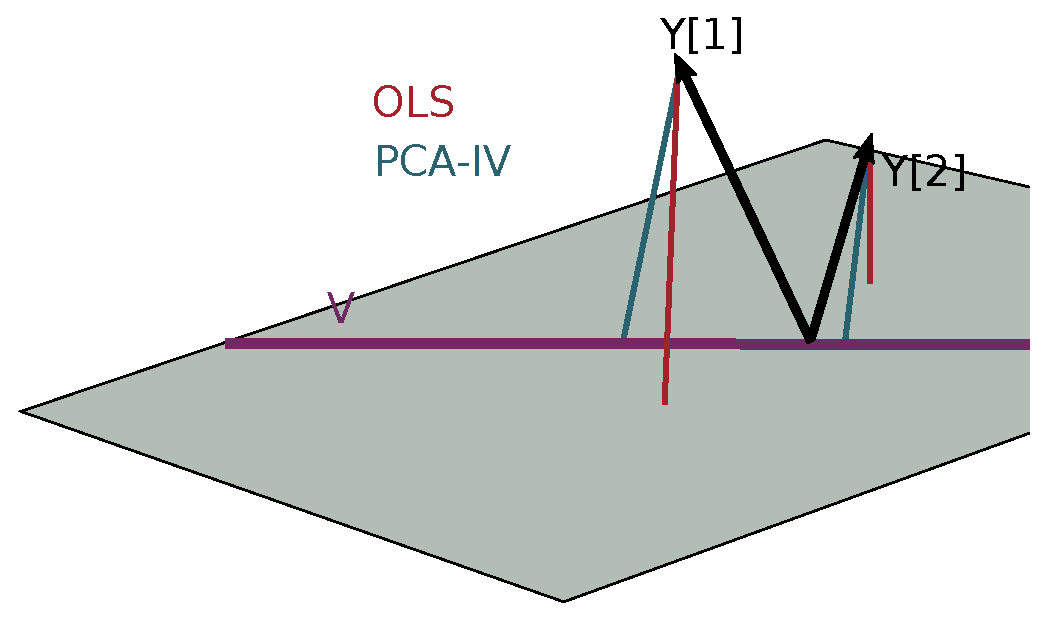
\includegraphics[width=0.7\textwidth]{figure/multitable/pca_iv/pca_iv_geometry}
  \caption{A geometric view of PCA-IV. The columns of the response $Y$ are views
    as $n$-dimensional vectors. The grey plane is the span of $X$. Multivariate
    OLS simply projects the columns of $Y$ onto the plane, while PCA-IV searches
    for a further subspace $V$ on which to project all
    responses. \label{fig:pca_iv_geometry} }
\end{figure}

Indeed, write the usual estimates for the covariance matrices of interest,
\begin{align*}
  \hat{\Sigma}_{YY} = \frac{1}{n}Y^{T}Y \\ \hat{\Sigma}_{YX} = \frac{1}{n}Y^{T}X
  \\ \hat{\Sigma}_{XX} = \frac{1}{n}X^{T}X
\end{align*}
and observe that the residual covariance of equation \ref{eq:pca_iv_resid_cov}
can be expressed
\begin{align*}
  &\frac{1}{n}\left[Y^{T}Y -
    Y^{T}XV\left(V^{T}X^{T}XV\right)^{-1}V^{T}X^{T}Y\right] \\ =
  &\frac{1}{n}\left[Y^{T}Y - Y^{T}Z\left(Z^{T}Z\right)^{-1}Z^{T}Y\right] \\ =
  &Y^T \left(I - P_{Z}\right)Y,
\end{align*}
where $P_{Z} = Z\left(Z^{T}Z\right)^{-1}Z^{T}$ is the projection operator onto
the columns of $Z$. Minimizing the trace of this matrix is equivalent to
minimizing
\begin{align*}
  \tr\left(Y^{T}\left(I - P_{Z}\right)Y\right) &= \tr\left(Y^{T}\left(I -
  P_{Z}\right)^{T}\left(I - P_{Z}\right)Y\right) \\ &= \|\left(I -
  P_{Z}\right)Y\|_{F}^{2} \\ &= \sum_{j = 1}^{p_{1}}\|\left(I -
  P_{j}\right)y_{\cdot j}\|^{2}_{2},
\end{align*}
which is exactly the sum of squared residuals from the columns of $Y$ onto the
span of the PCA-IV subspace, justifying the earlier geometric picture.

\subsubsection{Example}
\label{subsec:pcaiv_example}

Continuing our WELL-China case study, we now illustrate results from PCA-IV. The
idea of scores and loadings in this context requires some clarification. By
PCA-IV scores, we mean the coordinates of projections $z_{i}$ of samples onto
the subspace defined by $V$, and by loadings, we mean the correlation between
columns\footnote{Geometrically, the angle between original columns and the
  subspace, in the sense of Figure \ref{fig:pca_iv_geometry}.} of $X$ and $Y$
with the PCA-IV axes defining $V$.

We find that the scores, displayed in Supplementary Figures
\ref{fig:pca_iv_geometry} are similar to those that found by the concatenated
PCA of Section \ref{subsec:pca}. One possible explanation for this behavior is
that the PCA-IV generalized SVD of $X$ is similar to an ordinary PCA of $X$, and
that in the concatenated PCA of $\begin{pmatrix}Y & X\end{pmatrix}$, the fact
  that $X$ has many more columns than $Y$ means that the result is similar to a
  PCA on $X$ alone.

The loadings are given in Figure \ref{fig:pca_iv_loadings}. Interpretation of
the species loadings is simple, since species seem well separated by taxa.
Interpretation of the body composition variables is less clear -- pairs of
variables that would be expected to be near to one another are not, in many
cases. Indeed, leg fat mass (\texttt{leg\_fm}) and left leg fat mass
(\texttt{l\_leg\_fm}) should have a small angle between one another, but they do
not. It is possible that by approximating the covariation across tables, the
quality of within-table approximations deteriorates.

\begin{figure}
  \centering
  \includegraphics[width=\textwidth]{figure/multitable/pca_iv/loadings}
  \caption{The loadings for PCA-IV can be interpreted like loadings from
    previous methods, for example Figure \ref{fig:loadings}. Some of the
    relationships between variables seem less intuitive than those observed
    previously.
    \label{fig:pca_iv_loadings} }
\end{figure}

\subsection{Partial Triadic Analysis}
\label{subsec:partial_triadic_analysis}

Partial Triadic Analysis (PTA) gives an approach to working with multitable data
when each table has the same dimension, $p_1 = p_2$
\citep{leibovici1993facteurs, thioulouse2011simultaneous}. Specifically, it
gives a way of analyzing data of the form $\left(X_{\cdot\cdot l}\right)_{l =
  1}^{L}$, where each $X_{\cdot\cdot l} \in \reals^{n \times p}$. This is called
a data cube because it can also be written as a three-dimensional array $X \in
\reals^{n \times p \times L}$. We denote the $j^{th}$ feature measured on the
$i^{th}$ sample in the $l^{th}$ table by $x_{ijl}$, and the slices over fixed
$i$, $j$, and $l$ by $X_{i \cdot \cdot}$, $X_{\cdot j \cdot}$ and $X_{\cdot
  \cdot l}$. This type of data arises frequently in longitudinal data analysis,
where the same features are collected for the same samples over a series of $L$
times. However, the actual ordering of the $L$ tables is not ever used by this
method: if we scrambled the time ordering for $L$ tables, the algorithm's result
would not change.

The main idea in PTA is to divide the analysis into two steps,
\begin{itemize}
  \item Combine the $L$ tables into a single compromise table.
  \item Apply any standard single-table method, e.g., PCA, on the compromise
    table.
\end{itemize}

A naive approach to constructing the compromise table would be to average each
entry across the $L$ tables. Instead, PTA upweights tables that are more similar
to the average table, as these are considered more representative. Formally, the
compromise is defined as $X_c = \sum_{l = 1}^{L}\alpha_{l} X_{\cdot\cdot l} =
X\alpha \in \reals^{n \times p}$, where $\alpha$ (constrained to norm one) is
chosen to maximize $\sum_{l = 1}^{L} \alpha_{l} \left<\overline{X},
X_{\cdot\cdot l}\right>$, a weighted average of inner-products\footnote{We are
  using $\left<A, B\right> = \tr\left(A^{T}B\right)$.} between each of the $L$
tables and the naive-average table, $\overline{X} = \frac{1}{L}\sum_{l = 1}^{L}
X_{\cdot\cdot l}$.

The optimal $\alpha$ can be derived using Lagrange multipliers (see Supplemental
Section \ref{subsec:pta_alpha_derivation}), and leads to the compromise table,
\begin{align*}
  X_{c} = \sum_{l = 1}^{L} \frac{\left<\overline{X}, X_{\cdot\cdot
      l}\right>}{\sqrt{\sum_{l^{\prime} =1}^{L}\left<\overline{X}, X_{\cdot\cdot
        l^{\prime}}\right>^{2}}} X_{\cdot\cdot l}.
\end{align*}

We can try to interpret the compromise matrix geometrically. Suppose the
$X_{\cdot\cdot l}$ define an orthonormal basis, so that $\left<X^{l},
X^{l^{\prime}}\right> = \indic{l = l^{\prime}}$. Then, we can write the
compromise table as
\begin{align*}
  X_{c} = \sqrt{L}\sum_{l = 1}^{L}\left<\overline{X}, X_{\cdot\cdot
    l}\right>X_{\cdot\cdot l} = \sqrt{L}\overline{X},
\end{align*}
a scaled version of the mean.

If, however, the tables are not orthonormal, then we place more weight on
directions that are correlated. For example, if $X^{(1)} = X^{(2)}$, but the
rest of the tables are orthogonal to each other and to these first two tables,
then the compromise double counts the direction $X^{(1)}$. Therefore, compared
to the naive average $\overline{X}$, $X_c$ upweights more highly represented
tables.

\subsection{Statico and Costatis}
\label{subsec:statico_and_costatis}

In the multivariate ecology literature, it is common to have a pair of data
cubes, giving species abundances and environmental variables over time,
respectively. We write these as $Y \in \reals^{n \times p_{1} \times L}$ and $X
\in \reals^{n \times p_{2} \times L}$. Costatis and Statico are two approaches
for analyzing such data \citep{thioulouse2011simultaneous}. They are easiest to
understand as divide-and-conquer approaches, where the general problem of
analyzing a pair of data cubes is divided into two steps, one designed for
analyzing individual cubes, and another for studying covariation across tables.
In Statico, the covariation problem is dealt with first, then followed by a data
cube analysis, while in Costatis, that order is reversed.

Specifically, in Statico, an empirical cross-covariance matrix is constructed at
each time point, $Z^{l} = \frac{1}{n_{l}}Y^{T}_{\cdot\cdot l}X_{\cdot \cdot l}$.
For example, this is, the correlation between the environmental variables and
species counts at a specific timepoint $l$. The $L$ matrices $Z^{(l)}$ are then
input into a PTA, yielding a compromise table $Z_{c}$ which can then be studied
with PCA.

Alternatively, in Costatis, a compromise table is constructed for each of the
data cubes $Y$ and $X$, using PTA. Call these $Y_{c}$ and $X_{c}$. These are now
simply two matrices, each with $n$ rows, and they can be analyzed by any
two-table dimensionality reduction method, for example, CoIA.

Hence, we see that the only difference between these methods is the order in
which CoIA and PTA are applied. Indeed, this is reflected in the names of the
methods: Statis is an abbreviation for a PTA, and Statico performs a CoIA before
a Statis while Costatis does the reverse.

\subsection{Reduced-rank regression}
\label{subsec:label}

Reduced-rank regression is an approach to multiresponse regression which pools
information across responses \citep{izenman1975reduced, mukherjee2011reduced}.
Compared to performing separate regressions for each response, this pooling can
lead to meaningful performance improvements. Further, reduced-rank estimates can
often be more interpretable.

Suppose we have collected $p_{1}$ responses and $p_{2}$ features across $n$
samples, $y_{i} \in \reals^{p_{1}}$ and $x_{i} \in \reals^{p_{2}}$,
respectively. Our goal is to use this training data to predict the response
$y^{\ast}$ given a new sample $x^{\ast}$. Arrange these data into two matrices,
$Y \in \reals^{n \times p_{1}}$ and $X \in \reals^{n \times p_{2}}$.

The simplest approach to this problem is to fit a coefficient matrix $B \in
\reals^{p_{2} \times p_{1}}$ relating the $p_{2}$ features to the $p_{1}$
response coordinates by minimizing $\|Y - XB\|_{F}^{2}$. A slight modification
supposes that the responses might be correlated, and instead optimizes a
whitened version of the problem\footnote{This can also be viewed as using a
  Mahalanobis distance.}, $\|\left(Y -
XB\right)\hat{\Sigma}_{YY}^{-\frac{1}{2}}\|_{F}^{2}$

The optimal $B$ for these two approaches are $\left(X^{T}X\right)^{-1}X^{T}Y$
and $\left(X^{T}\hat{\Sigma}_{YY} X\right)^{-1}X^{T}\hat{\Sigma}_{YY}Y$
respectively. These simply concatenate coefficients from $p_{1}$ independent
linear regressions, one per response dimension.

This is not a very satisfactory solution, because we imagine there is
information to share across the different response dimensions: we should be able
to improve performance compared to parallel univariate regressions. Towards this
goal, consider that while there may be $p_{1}$ responses, their effective
dimension may be relatively low. Reduced-rank regression formalizes this with an
explicit constraint on the rank of $B$, defining an estimate
$\hat{B}^{\text{rr}}$ by the optimal value of
\begin{align}
\minimize_{B \in \reals^{p_{2} \times p_{1}}} &\|\left(Y -
XB\right)\Sigma_{YY}^{-\frac{1}{2}}\|_{F}^{2} \label{eq:rr_obj}\\ \text{such
  that } &\text{ rank}\left(B\right) \leq K, \nonumber
\end{align}
for some $K < p_{1}\wedge p_{2}$.

The optimal value is given by $\hat{B}^{\text{ols}}V_{K}V_{K}^{-}$, where the
columns of $V_{K}$ are the top $K$ response CCA directions and $V_{K}^{-}$
denotes the pseudoinverse of $V_k$. The derivation is provided in Supplementary
Section \ref{subsec:reduced_rank_derivation}.

Therefore $\hat{Y}^{\text{rr}} = X\hat{B}^{\text{rr}} = P_{X}YV_{k}V_{k}^{-}$,
which means that the reduced-rank fits can be obtained by first projecting the
columns of $Y$ onto the top $K$ response canonical directions, and then
projecting these pooled $Y$ onto the span of $X$. If the $Y$ had not been
pooled, then the projection onto the span of the $X$'s is exactly the
independent linear regressions. Hence, we have a clear geometric picture of the
effect of the reduced-rank constraint.

\section{Modern multivariate methods}

Compared to classical approaches, modern multivariate methods are typically
designed for more high-dimensional, heterogeneous settings. The two methods
reviewed in this section are examples of this trend: Partial Least Squares (PLS)
is well-suited for high-dimensional response matrices, while Canonical
Correspondence Analysis (CCpnA) was facilitates joint analysis of heterogeneous
continuous and count data necessary. Unlike traditional statistical methods,
neither approach is explicitly model-based, and both are iterative, requiring
more extensive computation than earlier techniques.

\subsection{Partial Least Squares}
\label{subsec:PLS}

PLS sequentially derives a set of mutually orthogonal features
$\left(z_{k}\right)_{k = 1}^{K}$ that characterizes the relationship between two
tables, $Y$ and $X$ \citep{wold1985partial}. To obtain the first PLS direction,
$z_{1}$, compute the first left singular vector $u_{1}$ of the cross-covariance
matrix between the two tables, $\hat{\Sigma}_{YX} = \frac{1}{n}Y^{T}X$. Then,
for each of the $p_{2}$ columns of $X$, compute the univariate (i.e., partial)
regression coefficient $\hat{\varphi}_{j}$ from the model $u_{1i} = \alpha_{0j}
+ \varphi_{j}x_{ij}$, for $i = 1, \dots, p_{1}$. The first PLS direction is
defined as $z_{1} = X\hat{\varphi}_{1}$. To generate subsequent directions,
orthogonalize both $Y$ and $X$ with respect to the current directions, and
repeat the process.

This procedure is appealing because, like PCA, it reduces a potentially
high-dimensional matrix $X$ with many correlated columns into a smaller set of
orthogonal directions. Moreover, it achieves this reduction in a way that
accounts for correlation with columns in $Y$: columns of $X$ that are
uncorrelated with $Y$ will have no contribution to the PLS directions, even if
they account for a large proportion of variation in $X$.

We have stated the procedure in the form it was originally proposed, but this
algorithmic description is difficult to understand geometrically or
probabilistically. However, statistical interpretations have since been
developed. \cite{frank1993statistical} and \cite{stone1990continuum} studied the
case where $p_{1} = 1$, so $y$ is a single column vector. By assuming that the
rows of $y$ and $X$ are drawn i.i.d. from distribution $\P^{YX}$, with marginals
$\P^{Y}$ and $\P^{X}$, they found that the $k^{th}$ PLS direction $z_{k}$ is the
$z$ that solves the optimization
\begin{align}
  \label{eq:pls_obj}
\maximize_{z} & \Corrsubarg{\P^{YX}}{x_{i}^{T}z_{k},
  y_{i}}\Varsubarg{\P^{X}}{z^{T}x_i} \\ \text{such that }&z^{T}X^{T}X z_{j} = 0
\text{ for all }j \nonumber \leq k - 1 \nonumber \\ \|z\|_2 = 1. \nonumber
\end{align}
If the covariance term is omitted, the optimization is identical to the maximum
variance problem that gives the principal component directions based on $X$.
This formulation makes precise the idea that PLS is a version of principal
components that accounts for correlation with $Y$. For $p_1 > 1$, this objective
can be generalized to the total covariance across response dimensions, $\sum_{j
  = 1}^{p_1} \Covsubarg{\P^{YX}}{x_i^T z_k, y_{ij}}$ \citep{chun2010sparse}.

An alternative interptetation, due to \citep{gustafsson2001probabilistic}, is
that PLS fits a particular latent variable model. Suppose $\xi_{i} =
\left(\xi_{i}^{s}, \xi_{i}^{X}\right)$ are drawn i.i.d. from a $K_{1} + K_{2} =
K$ dimensional spherical normal. PLS assumes the observed tables $Y$ and $X$
have rows drawn i.i.d. from
\begin{align*}
y_{i} \mid \xi_{i} &\sim \Gsn\left(\mu_Y + W_{Y}\xi_{i}^{s},
\sigma^{2}I_{p_{1}}\right) \\ x_{i} \mid \xi_{i} &\sim \Gsn\left(\mu_{X} + W_{X}
\xi_{i}^{s} + B_{X}\xi_{i}^{X}, \sigma^{2}I_{p_{2}}\right).
\end{align*}
That is, each table is the sum of two components, one that is a table-specific
linear combination of a shared latent variable, and another that is an arbitrary
linear combination of a table-specific latent variable. The shared feature
$\xi^{s}$ is the object of interest, and is what PLS implictly estimates.

\subsection{Sparse PLS}
\label{subsec:spls}

PLS suffers from two of the same problems as PCA,
\begin{itemize}
\item It can be unstable in high-dimensional settings, since it requires
  estimation of covariances, and isn't well defined when $p > n$.
\item PLS directions are linear combinations of all features in $x_i$, which can
  be difficult to interpret when there are many features.
\end{itemize}

Different regularized, sparse modifications of PCA have been proposed to remedy
these issues in the PCA context \citep{jolliffe2003modified, zou2006sparse,
  witten2009penalized}. For PLS, similar analysis leads to sparse PLS
\citep{le2008sparse, chun2010sparse}, and we briefly review this method here.

Directly regularizing the multiresponse version of the PLS optimization
\ref{eq:pls_obj} leads to the problem
\begin{align*}
  \maximize_{z_k} &\sum_{j = 1}^{p1} \Covsubarg{\P^{YX}}{x_i^T z_k, y_{ij}}
  \\ \text{such that }&z^{T}x^{T}x z_{j} = 0 \text{ for all }j \leq k - 1
  \\ &\|z_k\|_2 = 1 \\ &\|z_k\|_1 \leq \lambda,
\end{align*}
which can be applied to real data by replacing the objective with its sample
version, $z_k^{T} M z_k$, where $M = X^{T}YY^{T}X$. In this sample version, the
problem falls into the Penalized Matrix Decomposition framework of
\citep{witten2009penalized}, reviewed in Section \ref{subsec:pmd}.

However, \cite{chun2010sparse} argue that this formulation does not lead to
``sparse enough'' solutions. Instead, they adapt the SPCA approach of
\cite{zou2006sparse} to PLS. The resulting objective identifies two sets of
directions, a set $\left(a_k\right)$ that maximize the PLS-defining covariance
and another, $\left(z_k\right)$, that approximates the first set by a sparser
alternative. Formally, consider
\begin{align}
  \label{eq:spls_obj}
  \minimize_{z_k, a_k} &-\kappa \|a_k\|_M^2 + \left(1 - \kappa\right) \|z_k -
  a_k\|_M^2 \\ \text{ such that } & \|a_k\|_2^2 = 1 \nonumber \\ &\|z_k\|_1 \leq
  \lambda_1 \nonumber \\ &\|z_k\|_2 \leq \lambda_2, \nonumber
\end{align}
where we have defined $\|x\|_M = \sqrt{x^T M x}$ and $\kappa, \lambda_1$, and
$\lambda_2$ are tuning parameters. The first term in the objective is the
PLS-defining covariance, the second ensures that the solutions $z_k$ and $a_k$
are similar, and the norm constraints induce sparsity and stability on $z_k$.
$\kappa$ trades off the importance of the two components of the objective. Note
that while this objective is not convex, for fixed $a_k$, it is an elastic-net
regression, while for fixed $z_k$, it is a type of eigenvalue problem.

To develop some intuition for this optimization problem, we review the
motivation behind the analogous sparse PCA objective. Suppose we have the SVD,
$X = UDV^T$. It is a simple observation that the $k^{th}$ principal component is
proportional to the solution of a ridge regression onto $y_k = u_k d_k$,
\begin{align*}
  \hat{v}_k &\propto \arg \min_{v_k} \|y_k - X v_k\|_2^2 + \lambda \|v_k \|_2.
\end{align*}
Indeed, according to the usual ridge regression formula, the minimizer is
\begin{align*}
  \left(X^TX + \lambda I\right)^{-1} X^T y_k &= \left(V^T D^2 V + \lambda
  I\right)^{-1} V D U^T u_k d_k \\ &= V\left(D^2 + \lambda I\right)^{-1} D e_k
  d_k \\ &= \frac{d_k^2}{d_k^2 + \lambda}v_k.
\end{align*}

A less obvious fact is that still this connection between PCA continues to hold
even without direct access to the $u_k$ and $d_k$. Indeed, it turns out that in
the problem
\begin{align}
  \label{eq:spca_obj_reform}
  \text{minimize}_{A, V} &\sum_{i = 1}^{n} \|x_i - AV^T x_i\|_2^2 + \lambda
  \sum_{k = 1}^{K} \|v_k\|_2 \\ \text{subject to } &A^T A = I_K, \nonumber
\end{align}
the optimal $\hat{V}$ corresponds exactly to the top $K$ right singular vectors
of $X$. The idea of \cite{zou2006sparse} is to induce sparsity on $v_k$ by
constraining their $\ell^1$ norm, resulting in sparse principle component
directions. The objective \ref{eq:spls_obj} is the analog of this problem when
setting $z_k = v_k$, $\kappa = \frac{1}{2}$ and $M = X^T X$.

Reformulating the optimization \ref{eq:spca_obj_reform} suggests a simple
algorithm for solving it. First, notice that if we extend $\tilde{A}
= \begin{pmatrix} A & A^{\perp}\end{pmatrix}$ so that it is orthonormal, then
since norms are preserved under orthonormal rotations,

\begin{align*}
  \sum_{i = 1}^{n} \|x_i - AV^T x_i\|_2^2 &= \|X - XVA\|_{F}^2 \\ &=
  \|\begin{pmatrix} XA - XV \\ XA^{\perp} \end{pmatrix} \|_{F}^2 \\ &=
  \|\begin{pmatrix} XA - XV \\ XA^{\perp} \end{pmatrix} \tilde{A} \|_{F}^2 \\ &=
  \sum_{k = 1}^{K} \|Xa_k - X v_k\|_2^2 + C
\end{align*}
where $C$ is constant in $A$, and hence the sparse PCA objective can be written
as
\begin{align*}
  \text{minimize}_{A, V} &\sum_{k = 1}^{K} \|Xa_k - X v_k\|_2^2 + \sum_{k =
    1}^{K} \lambda_2 \|v_k\|_2 \\ \text{such that }&\|a_k\|_2 = 1 \\ & \|v_k\|_1
  \leq \lambda_1 \\ &A^TA = I_K.
\end{align*}
For a fixed $A$, this is an elastic-net regression. For fixed $V$, considering
that $\sum_{k = 1}^{K} \|Xa_k - Xv_k\|^2_2 = \|XA - XV\|_F^2$, this is a
Procrustes rotation problem. Hence, a local minimum can be found by alternating
these two steps until convergence.

\subsubsection{Example}
\label{subsubsec:spls_example}

Next we apply the SPLS implementation of \cite{chung2012spls} to the WELL-China
body composition data. We use the body composition variables as the response $Y$
and the microbiome community composition as $X$. We subset to female subjects
and filter species according to a $K$-over-$A$ filter with $K$ = 7\% of samples
and $A = 5$. This leaves 372 species over 119 participants. All species
abundances are variance-stabilized using the approach of
\cite{anders2010differential}. We cross-validate with 5 folds, searching through
a grid over $K \in \{4, \dots, 8\}$ and $\lambda_1 \in \{0, 0.05, \dots, 0.7\}$.
This grid is used to prevent the model from regularizing to the point that there
is no information to visualize. For example, if we set $K = 1$, every row of
Figure \ref{fig:spls_coef_heatmap} would look identical. The predictive accuracy
is poor, which is unsurprising considering the spike at 0 in the abundances
histogram -- the held out error is $\approx 1.29$, after having scaled and
centered the body composition variables.

Figure \ref{fig:spls_coef_heatmap} displays fitted coefficients relating body
composition variables with species abundances. By fitted coefficients, we mean
we display $\hat{B} = ZQ^T$, where $Z$ are the SPLS directions and a
multiresponse linear regression model is used, $Y = XB + E = XZQ^T + E$.
Positive associations tend to occur across all responses simultaneously, while
negative associations can be unique to either lean or fat mass. Most taxonomic
families seem to have slightly more negative than positive associations, with
the possible exception of Porphyromonodaceae.

\begin{figure}
  \centering
  \includegraphics[width=\textwidth]{figure/multitable/spls/coef_heatmap}
  \caption{ Coefficients learned by SPLS. Each row is a response dimension,
    which is a body composition variable. Each column is associated with a
    species. The shading within each cell corresponds to the SPLS coefficient
    for that species-response pair. Green and purple cells are positive and
    negative coefficients, respectively. Species are grouped first according to
    their taxonomic family, marked by grouping panel colors, and then by a
    hierarchical clustering on coefficient values.
    \label{fig:spls_coef_heatmap} }
\end{figure}

To interpret these coefficients in the raw data, we can visualize individual
species with strong associations to body composition. Specifically, we study
associations with the android and gynoid fat mass variables. In Figures
\ref{fig:spls_android_fm_species} and \ref{fig:spls_gynoid_fm_species}, we
display the abundances $X$ for species against android and gynoid fat mass,
respectively. The species are chosen according to whether the two-dimensional
coefficient across android and gynoid fat mass has large
norm\footnote{Specifically, $\left\| \begin{pmatrix} \beta_{android}
    \\ \beta_{gynoid} \end{pmatrix} \right\|_{2} > 0.065$.}. The main
associations that are visible are those between the body composition and species
presence or absence. That is, there don't seem to be any cases where a body
composition feature varies smoothly as a species becomes more or less abundant.
Instead, SPLS has identified species whose samples have lower or higher android
or gynoid fat mass, depending on whether that species is present or absent. This
suggests that a logistic regression version of SPLS \citep{chung2010sparse},
applied to the presence-absence transformed version of this data may fit the
data just as well, with the advantage of being somewhat more interpretable.

\begin{figure}
  \centering
  \includegraphics[width=\textwidth]{figure/multitable/spls/android_fm_species}
  \caption{A subset of the species whose coefficients for total lean and fat
    mass are high in magnitude. Each panel represents one species, and each
    point is a samples $\times$ species combination. The $x$-axis gives the
    abundance of that species across samples, and the $y$-axis gives android fat
    mass of the associated sample. Colors indicate taxonomic family membership.
    Panels are sorted from most positive to most negative association. Within
    each panel, a linear smooth is given, independent of the estimated
    coefficient.
    \label{fig:spls_android_fm_species} }
\end{figure}


\begin{figure}
  \centering
  \includegraphics[width=\textwidth]{figure/multitable/spls/gynoid_fm_species}
  \caption{ The analog of Figure \ref{fig:spls_android_fm_species}, but with
    gynoid, rather than android, fat mass along the
    $y$-axis. \label{fig:spls_gynoid_fm_species} }
\end{figure}

\subsection{CCpnA}
\label{subsec:canonical-correspondence}

CCpnA is a method, originally developed in ecology, useful for joint analysis of
count and continuous data. The canonical application has a site by species count
matrix $Y \in \reals^{n \times p_{1}}$ and an environmental features matrix $X
\in \reals^{n \times p_{2}}$, for example, historical rainfall and temperature
measurements. The scientific goal might be to identify species that are more
abundant in sites with more rainfall or higher temperature. If these
environmental variables were uncorrelated, it would be enough to fit a separate
regression to each. This however is rarely the case, motivating the development
for CCpnA.

CCpnA produces low-dimensional representations of both the rows and columns of
$Y$ (the sites and species), along with latent subspaces on which these
representations are defined. Algorithmically, CCpnA first constructs the
following matrices, where $1_{r}$ denotes a column vector of $r$ ones,
\begin{enumerate}
  \item An overall frequency matrix,
    \begin{align*}
      F = \frac{1}{n_{\cdot\cdot}^{Y}} Y,
  \end{align*}
  where $n_{\cdot\cdot}^{Y}$ is the sum of all counts in matrix $Y$.
\item A diagonal matrix of row (site) proportions,
  \begin{align*}
    D_{r} &= \diag\left(F 1_{p_{1}}\right) \in \reals^{n \times n}.
  \end{align*}
\item A diagonal matrix of column (species) proportions,
  \begin{align*}
    D_{c} &= \diag\left(F^{T}1_{n}\right) \in \reals^{p_{1} \times p_{1}}.
  \end{align*}
\item A projection onto the columns of the environmental matrix $X$, reweighting
  sites according to their species counts,
  \begin{align*}
    P_{X} &=
    D_{r}^{\frac{1}{2}}X\left(X^{T}D_{r}X\right)^{-1}X^{T}D_{r}^{\frac{1}{2}}
    \in \reals^{n \times n}.
\end{align*}
\end{enumerate}

With this notation, compute an SVD,
\begin{align*}
D_{r}^{-\frac{1}{2}}\left(F - F 1_{p}1_{p}^{T}F\right)D_{c}^{-\frac{1}{2}}P_{X}
= UDV^{T},
\end{align*}
and define row and column scores $Z$ and $Q$ by
\begin{align*}
  Z &= D_{r}^{-\frac{1}{2}} UD \\ Q &= D_{c}^{-\frac{1}{2}}V^{T}D.
\end{align*}

There are several ways to interpret this procedure. CCpnA was originally
proposed as the solution to a fixed-point iteration called reciprocal averaging
\citep{ter1986canonical}. Later, \cite{greenacre1987geometric,
  greenacre1984theory}, provided a geometric view and \cite{zhu2005constrained}
gave an exact probabilistic interpretation.

The intuition for the reciprocal averaging procedure is simple: the scores for
different sites should be a weighted average of the species scores, with larger
weights for the species that are more common at those sites. Similarly, species
scores can be defined according to a weighted average of site scores. That is,
\begin{align*}
  z_{i} \propto \frac{1}{f_{i\cdot}}\sum_{j = 1}^{p_{1}}f_{ij}q_{ij} \\ q_{j}
  \propto \frac{1}{f_{\cdot j}} \sum_{i = 1}^{n} f_{ij}z_{ij},
\end{align*}
or, in matrix form,
\begin{align*}
Z \propto \diag\left(F 1_{p}\right)^{-1} F Q^{T} \\ Q \propto \diag\left(F^{T}
1_{n}\right)^{-1} Z.
\end{align*}
This formulation suggests an algorithm for finding $Z$ and $Q$ -- arbitrarily
initialize one and iterate these calculations until convergence.

As is, this is not yet the setup that yields CCpnA\footnote{It in fact gives the
  solution to the Correspondence Analysis problem (the similarity is the reason
  for the name Canonical \textit{Correspondence Analysis}).} -- it doesn't use
information in the environmental table $X$. To recover CCpnA, a projection step
needs to be inserted before the calculation of row scores,
\begin{enumerate}
\item Arbitrarily initialize $Z$.
\item While not converged,
\begin{enumerate}
\item Solve $Q^{\prime} \propto \diag\left(F^{T}1_{n}\right)^{-1}F^{T}Z$.
\item Project $Q = P_{X}Q^{\prime}$.
\item Solve $Z \propto \diag\left(Z 1_{p}\right)^{-1} F Q^{T}$.
\end{enumerate}
\end{enumerate}

The fixed point of this iteration is the previously described CCpnA solution.

A second interpretation is due to \cite{zhu2005constrained}. Suppose first that
we are only interested in a one-dimensional score for rows and columns. Let
$\alpha$ be a latent environmental gradient, for example, between warm-dry and
cold-wet sites. For each of the $p_{1}$ species, define a normal density over
the environmental variables, $f_{j}\left(x_{i}\right) = \Gsn\left(x_i \vert
\mu_{j}, \Sigma_{j}\right)$. The mode of this density represents the preferred
environment for species $j$. Next, project these densities onto the
environmental gradient, giving a univariate $f_{j}^{\alpha}\left(z_{i}\right) =
\Gsn\left(z_i \vert \alpha^{T}\mu_{j}, \alpha^{T} \Sigma_{j}\alpha\right)$ for
each species. The $z_{i}$ represent the scores for species $i$ along the
environmental gradient $\alpha$.

The generative model views species-site pairs one at a time. For each pair
involving site $i$ and species $j$, draw a score according to
$f_{j}^{\alpha}\left(z_{i}\right)$. Hence, each site $i$ draws species according
to a $p_{1}$-class LDA model.

To use this idea to compute scores, we need to estimate the environmental
gradient $\alpha$, which is also of interest in its own right. This is done by
supposing equal covariances across species, $\Sigma_{j} = \Sigma$ for all $j$,
and finding the $\hat{\alpha}$ maximizing the between vs. total variance across
species,
\begin{align*}
  \frac{\alpha^{T} \Sigma_{B} \alpha}{\alpha^{T} \Sigma \alpha},
\end{align*}
where
\begin{align*}
  \Sigma_{B} = \sum_{j = 1}^{p_{1}} f_{\cdot j}\left(\mu_{j} -
  \bar{\mu}\right)\left(\mu_{j} - \bar{\mu}\right)^{T}
\end{align*}
is a between species covariance matrix. Estimating $\hat{\alpha}$ in this way
and writing $z_{i} = \hat{\alpha}^{T}x_{i}$ gives the original site scores from
CCpnA.

\subsection{Kernel CCA}
\label{subsec:kernel_cca}

Since CCA is based on correlation, it can only summarize linear relationships
across tables -- Kernel CCA (KCCA) is a modification that is sensitive to
nonlinear associations \citep{akaho2006kernel, bach2003kernel,
  lanckriet2004statistical}. It does this by implicitly lifting the original
data into a richer feature space, with the hope that nonlinear associations in
the original data become linear associations in the richer space -- this is
often called the ``kernel trick'' \citep{scholkopf2001kernel}. Informaly, KCCA
is the algorithm that emerges after applying the kernel trick to CCA.

More precisely, let $\varphi^{Y}: \reals^{p_{1}} \to H^{Y}$ and $\varphi^{X}:
\reals^{p_{2}} \to H^{X}$ be mappings from the features directly measured by $X$
and $Y$ into richer spaces $H^{Y}$ and $H^{X}$. For example, the $\varphi$ might
map vectors into an expansion of all polynomial products of original feature
values, up to some fixed degree, this mapping is called the polynomial kernel.
As in CCA, let $\P^{YX}$ denote the sampling distributions associated with the
two tables, and write $x_{i}$ and $y_{i}$ for generic draws from these
distribution.

In the same way that the first CCA direction maximizes the covariance between
linear combinations $u^{T}x_{i}$ and $v^{T}y_{i}$, KCCA maximizes the
correlation between the more general inner products, $z_{i}\left(u\right) =
\left<u, \varphi\left(x_{i}\right)\right>$ and $z_{i}\left(v\right) = \left<v,
\varphi\left(y_{i}\right)\right>$,
\begin{align}
  \argmax_{u \in H^{X}, v \in H^{Y}} &\Covsubarg{\P^{YX}}{z_{i}\left(u\right),
    z_{i}\left(v\right)} \label{eq:optim_kcca}\\ \text{subject to }
  &\Varsubarg{\P^{X}}{z_{i}\left(u\right)} =
  \Varsubarg{\P^{Y}}{z_{i}\left(v\right)} = 1. \nonumber
\end{align}

As is, the problem is not well-posed, and it is necessarily to regularize. The
regularized Lagrangian associated with the optimization in equation
\ref{eq:optim_kcca} is
\begin{align}
  &\Covsubarg{\P^{YX}}{z_{i}\left(u\right), z_{i}\left(v\right)} -
  \frac{\rho^{X}}{2}\Varsubarg{\P^{X}}{z_{i}\left(u\right)} -
  \frac{\rho^{Y}}{2}\Varsubarg{\P^{Y}}{z_{i}\left(v\right)}
  + \label{eq:lagrangian_kcca}\\ &\frac{\lambda^{X}}{2}\text{Pen}\left(u\right)
  + \frac{\lambda^{Y}}{2}\text{Pen}\left(v\right), \nonumber
\end{align}
where $\text{Pen}\left(x\right)$ is some regularizer, the $\ell^{1}$ or
$\ell^{2}$ norm, for example.

The optimal $u$ and $v$ must lie in the spans of
$\left(\varphi^{X}\left(x_{i}\right)\right)_{i =1 }^{n}$ and
$\left(\varphi^{Y}\left(y_{i}\right)\right)_{i =1 }^{n}$, respectively, since
directions orthogonal to these subspaces cannot improve the correlation in the
objective. Therefore,
\begin{align*}
u &= \Phi^{X} \alpha^{X} \\ v &= \Phi^{Y} \alpha^{Y},
\end{align*}
for some $\alpha^{X}, \alpha^{Y}$, where $\Phi^{X} \in \reals^{n \times
  \text{dim}\left(H^{X}\right)}$ has $i^{th}$ row
$\varphi^{Y}\left(x_{i}\right)$ and $\Phi^{Y}$ is defined similarly.

Substituting this into the Lagrangian in equation \ref{eq:lagrangian_kcca}, it
becomes clear that only the cross-products ${\Phi^X}^{T}\Phi^{X}$ and
${\Phi^{Y}}^{T} \Phi^{Y}$ appear. Since these inner products can be written as
kernel matrices -- call them $K^{X}$ and $K^{Y}$ -- the optimization can be
fully expressed in terms of kernels, without reference to the original $X$ or
$Y$. It can then be shown that the optimal $\alpha^{X}$ and $\alpha^{Y}$ are the
solutions to the generalized eigenvalue problem,
\begin{align*}
  \begin{pmatrix}
    0 & K^{X}K^{Y} \\ K^{Y}K^{X} & 0
  \end{pmatrix}
  \begin{pmatrix}
    \alpha^{X} \\ \alpha^{Y}
  \end{pmatrix}
&= \rho
\begin{pmatrix}
  \left(K^{X} + \lambda^{X}I_{p_{1}}\right)^{2} & 0 \\ 0 & \left(K^{Y} +
  \lambda^{Y}I_{p_{2}}\right)^{2}
\end{pmatrix}
\begin{pmatrix}
  \alpha^{X} \\ \alpha^{Y}
\end{pmatrix}.
\end{align*}
A geometric interpretation of Kernel CCA is given in \cite{kuss2003geometry},
which translates the Euclidean picture associated with CCA to the more general
RKHS setting. Often, however, KCCA results can be difficult to use in
exploratory analysis, because only sample scores are provided. Eigenvectors are
never computed in the spaces $H^{X}$ and $H^{Y}$, so it's not possible to make a
biplot. Consequently, KCCA scores are typically interpreted using supplementary
characteristics of the samples.

\subsection{Penalized Matrix Decomposition}
\label{subsec:pmd}

In high-dimensional settings, sparsity is a desirable property, both for
qualitative interpretability and statistical stability. A regression model using
only a few features is easier to understand than one involving a linear
combination of all possible features. Further, regularized models typically
outperform their unregularized counterparts in terms of both predictive accuracy
and inferential power \citep{buhlmann2011statistics}. In fact, it is impossible
to fit a unregularized linear regression when the number of features is greater
than the number of samples.

The Penalized Matrix Decomposition (PMD) is a general approach to adapting the
reguarlization machinery developed around regression to the multivariate
analysis setting \citep{witten2009penalized}. The CCA and MultiCCA instances of
PMD have been particularly well-studied \citep{witten2009penalized,
  witten2013package}.

The general setup is as follows. Suppose we want a one-dimensional
representation of the samples (rows) in $X \in \reals^{n \times p}$. Recall that
the first $k$-eigenvectors recovered by PCA span a subspace that minimizes the
$\ell^{2}$-distance from the original data to their projections onto that
subspace. In particular, when $k = 1$, the associated PCA coordinates $u \in
\reals^{n}$ and eigenvector $v$ are the optimal values in the problem
\begin{align*}
  \minimize_{u \in \reals^{n}, v \in \reals^{p}, d \in \reals} &\|X -
  duv^{T}\|_{2}^{2} \\ \text{subject to } &\|u\|_{2}^{2} = \|v\|_{2}^{2} = 1.
\end{align*}

\begin{figure}
  \centering
  \includegraphics[width=\textwidth]{figure/multitable/pmd/illustration_sequence}
  \caption{An example of the PMD CCA solution in a high-dimensional source
    separation problem, based on the simulation experiment in
    \citep{witten2009penalized}. The solid lines indicate true ``sources''
    underlying observed data tables $X \in \reals^{20 \times 504}$ and $Y \in
    \reals^{20 \times 504}$. Specifically, $X$ and $Y$ are defined as random
    linear combinations of two sources each, which are then corrupted with
    noise. The recovered sources from CCA between $X$ and $Y$ using a
    fused-lasso penalty are plotted as points. The fused-lasso regularization
    parameter was chosen by cross-validation. The long flat lines in the
    recovered solutions reflect this penalty. Note that PMD is able to recover
    the positions at which changepoints in the source signal occur, but that
    sources are nonidentifiable without further constraints. Further, in the
    table $X$, a region with truly zero signal is estimated very poorly, for
    reasons that are unclear. A scatterplot view of this same data is provided
    in Figure
    \ref{fig:pmd_illustration_scatter}. \label{fig:pmd_illustration_sequence}}
\end{figure}

The PMD generalizes this formulation of rank-one PCA to enforce additional
structure on $u$ and $v$. The PMD solutions $u$ and $v$ are defined as the
optimizers of
\begin{align}
\label{eq:pmd_opt} \minimize_{u \in \reals^{n}, v \in \reals^{p}, d
  \in \reals} &\|X - duv^{T}\|_{2}^{2} \\ \text{subject to } &\|u\|_{2}^{2} =
\|v\|_{2}^{2} = 1 \nonumber \\ & \text{Pen}_{u}\left(u\right) \leq \mu_{1}
\nonumber \\ & \text{Pen}_{v}\left(v\right) \leq \mu_{2}, \nonumber
\end{align}
where $\text{Pen}_u$ and $\text{Pen}_v$ are arbitrary constraints on $u$ and
$v$.

To choose the regularization parameters $\mu_{1}$ and $\mu_{2}$,
\citep{witten2009penalized} applied cross-validation to the reconstruction
errors after holding out random entries in $X$. To obtain a sequence of scores
and eigenvectors $\left(u_{k}\right)_{k = 1}^{K}$ and $\left(v_{k}\right)_{k =
  1}^{K}$ for $K > 1$, define $u_{k}$ and $v_{k}$ as the optimizers of the
problem \ref{eq:pmd_opt} on the residual: $X^{k} := X^{k - 1} - d_{k - 1}u_{k -
  1}v_{k - 1}^{T}$ where $d_{k} = u_{k}^{T} X^{k}v_{k}$ and $X^{1} = X$. The
effect of regularization is illustrated in Figure
\ref{fig:pmd_illustration_sequence}.

%% (todo: geometric interpretation)
%% (todo: generalized least squares / probabilistic interpretation
%% \cite{allen2014generalized})

This view can be specialized to develop regularized versions of a number of
multivariate analysis problems. We consider applications to the CCA and MultiCCA
problems. Recalling that $\|A\|_{F}^{2} = \tr\left(A^{T}A\right)$ along with the
linearity and the cyclic properties of the trace, the objective in
\ref{eq:pmd_opt} can be rewritten, using $\equiv$ to mean equality up to terms
constant in $u$ and $v$,
\begin{align*}
  \|X - duv^{T}\|_{F}^{2} &= \tr\left(\left(X - duv^{T}\right)^{T}\left(X -
  duv^{T}\right)\right) \\ &\equiv -2d\tr\left(X^{T}uv^{T}\right) +
  d^{2}tr\left(uv^{T}vu^{T}\right) \\ &\equiv -2d v^{T}X^{T}u + d^{2}
\end{align*}
where for the last equivalence we used that $v^{T}v = u^{T}u = 1$.

From this expression, and by partially minimizing out $d = v^{T}X^{T}u$, we see
that the PMD solutions $u$ and $v$ in \ref{eq:pmd_opt} can be found as the
optimizers of
\begin{align}
\label{eq:pmd_reform}  \maximize_{u \in \reals^{n}, v \in \reals^{p}} \medspace &u^{T}X^{T}v \\
  \text{subject to } &\|u\|_{2}^{2} = \|v\|_{2}^{2} = 1 \nonumber
  \\ &\text{Pen}_{u}\left(u\right) \leq \mu_{1}\nonumber
  \\ &\text{Pen}_{v}\left(v\right) \leq \mu_{2} \nonumber
\end{align}

Notice that, as long as the penalties are convex in $u$ and $v$, the
optimization is biconvex, so a local maximum can be found by alternately
maximizing over $u$ and $v$.

From this form, we can derive a sparsity-inducing version of CCA. Recall the
maximal-covariance interpretation of CCA,
\begin{align*}
  \maximize_{u \in \reals^{p_{1}}, v \in \reals^{p_{2}}} \medspace
  &u^{T}\hat{\Sigma}_{XY}v \\ \text{subject to } &u^{T}\hat{\Sigma}_{XX} u = v^{
    T}\hat{\Sigma}_{YY}v = 1.
\end{align*}

\citep{witten2009penalized} argues for diagonalized CCA, in which the variance
constraints are replaced by unit norm constraints, and sparsity-inducing
$\ell^{1}$-constraints are added,
\begin{align*}
  \maximize_{u \in \reals^{p_{1}}, v \in \reals^{p_{2}}} & u^T\hat{\Sigma}_{XY}v
  \\ \text{subject to } &\|u\|_{2}^{2} = \|v\|_{2}^{2} = 1 \\ &\|u\|_{1} \leq
  \mu_{1} \\ &\|v\|_{1} \leq \mu_{2}
\end{align*}
which is exactly of the form of equation \ref{eq:pmd_reform} where $X =
\hat{\Sigma}_{XY}$.

Multiple CCA can also be described in this framework, by replacing the objective
with the sum over all pairwise covariances, $\sum_{l, l^{\prime} = 1}^{L}
c_{1}^{(l) T}X^{(l) T}X^{(l^{\prime})}c_{1}^{(l)^{\prime}}$, and introducing
constraints for each of the $c_{1}^{(l)}$.

\subsubsection{Example}
\label{subsec:sparse_cca_example}

We apply the PMD formulation of sparse CCA to the WELL-China data. As before, we
$k$-over-$A$ filter the microbiome data, requiring species to have counts of at
least 5 in at least 7\% of samples. Further, we first variance-stabilize,
center, and scale these species abundances. For the regularization parameters,
we set $\mu_1 = 0.7$ for the body composition data and $\mu_2 = 0.3$ for the
species count data. Our reasoning is that sparsity within species loadings is
more important than sparsity across body composition variables, because the
microbiome data is more high-dimensional. We only compute the first three PMD
directions, and the associated correlations between scores are $\left(d_1, d_2,
d_3\right) = \left(0.700, 0.435, 0.632\right)$. Note that the correlation can
increase in subsequent directions, since directions are computed iteratively,
and cannot be defined and sorted all at once.

The learned loadings and scores are displayed in Figures \ref{fig:pmd_loadings}
and \ref{fig:pmd_scores_android_fm}, respectively. The $x$-axis in the loadings
differentiates between high android and gynoid fat mass. The $y$-axes in the
loadings reflect a gradient between overall right and left body mass. The size
of points corresponds to the third PMD direction, and it seems to highlight high
BMI, ratio of fat to lean mass, and overall weight. We interpret species based
on their positions relative to these body composition variables, as in an
ordinary biplot. For example, species 271 seems to be more common among people
with higher android and lower gynoid fat mass.

The associated scores are displayed in Figure \ref{fig:pmd_scores_android_fm},
shaded in according to android fat mass. The gradient between android and gynoid
fat mass suggested by the loadings is clearly visible from this display. The
length of links reflects the correlation between sets of scores. They are
somewhat longer in the sparse CCA compared to the ordinary CCA on a subset of
species, but this is likely a consequence of regularization and overfitting on
the part of ordinary CCA.

\begin{figure}
  \centering \includegraphics[width=\textwidth]{figure/multitable/pmd/loadings}
  \caption{ Body composition and species loadings produced by sparse CCA, for
    variables with at least one nonzero coordinate. Each point corresponds to a
    species loading, and is shaded in by taxonomic family. Species with loadings
    far from the origin are also annotated with their names. Black text are
    loadings for body composition variables. The size of points and text
    reflects the contribution of the third CCA dimension. Many loadings have at
    least one dimension that is exactly zero, due to $\ell^{1}$-regularization.
    There appear to be a gradient with android and gynoid weight, running from
    left to right, and this is confirmed in Figures
    \ref{fig:pmd_scores_android_fm} and \ref{fig:pmd_android_fm_species}.
    \label{fig:pmd_loadings}
  }
\end{figure}

\begin{figure}
  \centering
  \includegraphics[width=\textwidth]{figure/multitable/pmd/scores_android_fm}
  \caption{ Sample scores provided by sparse CCA. Each point is a sample,
    positioned at their coordinates with respect to the first two learned sparse
    CCA directions. Points are shaded in according to android fat mass, and
    their sizes are set according to the third sparse CCA direction's
    contribution. Evidently, the first two directions reflect a gradient across
    android fat mass, suggesting that this is a substantial contributor to
    covariation across microbiome and body composition tables.
    \label{fig:pmd_scores_android_fm}
  }
\end{figure}

We can folow-up these displays by focusing on species that seemed related to the
CCA axes. In Figure \ref{fig:pmd_android_fm_species}, we isolate species with
loadings a distance of at least 0.15 from the origin. These are the same ones
that are labeled by text in Figure \ref{fig:pmd_loadings}. We can see
associations between abundance and android fat mass, as suggested by the
loadings. Generally, there is a difference between android fat mass among people
with and without particular species -- there is generally no smooth function
between the quantity of a species android fat mass, even in these cases where an
association exists. Further, no individual taxonomic group seems to dominate the
set of associated species. Instead, a few isolated members of a few different
taxonomic groups seem to be associated with android fat mass.

\begin{figure}
  \centering
  \includegraphics[width=\textwidth]{figure/multitable/pmd/android_fm_species}
  \caption{ A more focused view of the species with high loadings in Figure
    \ref{fig:pmd_loadings}. Each panel corresponds to a species. Points are
    shaded in according to each species' taxonomic family. The $x$-axis within
    panels corresponds to variance-stabilized species abundance, while the
    $y$-axis gives android fat mass. A linear smooth is provided to summarize
    the direction of associations. Panels are arranged according to the size of
    that species' loading onto the first sparse CCA axis. The presence of
    certain species seems to correspond to increased or decreased levels of
    android fat mass.
    \label{fig:pmd_android_fm_species}
  }
\end{figure}

\subsection{Multitable Mixed-Membership}
\label{subsec:multitable_mixed_membership}

In Section \ref{subsec:cca}, a latent variable interpretation of CCA was
provided as an alternative to the standard covariance maximization perspective.
Since likelihood based methods are easily adapted to different data types, it is
natural to consider versions of CCA designed for non-Gaussian data, using
Section \ref{subsec:cca} as a starting point. We are particularly interested in
data with the same structure as the WELL-China body composition and microbiome
data, namely two table data where one table is continuous with Gaussian
marginals and correlated columns and the other is a high-dimensional collection
of counts, where many entries are exactly zero.

As before, define a set of shared scores $\xi_{i}^{s} \in \reals^{K}$, and two
sets of within-table scores, $\xi_{i}^{X} \in \reals^{L_{1}}$ and $\xi_{i}^{Y}
\in \reals^{L_{2}}$. As before, we model the body composition variables using a
essentially a Gaussian factor analysis model, $y_{i} \vert \xi_{i}^{X},
\xi_{i}^{Y} \sim \Gsn\left(B^{y}\xi_{i}^s + W^y \xi_{i}^y,
\sigma^{2}I_{p_{2}}\right)$ with a spherical Gaussian prior on $\xi_{i}^{X},
\xi_{i}^{Y}$. For the counts matrix, we might consider a few different
approaches,

\begin{itemize}
\item Bayesian Exponential Family PCA \citep{mohamed2009bayesian}: By requiring
  low-rank structure on the natural parameters of an exponential family model,
  we could naturally model high-dimensional count data, using a Poisson or
  multinomial likelihood, for example.
\item Nonnegative Matrix Factorization \citep{lee2001algorithms}: A variant of
  the exponential family approach is to model the counts matrix as a Poisson
  likelihood over a low-rank product of Gamma random matrices.
\item Latent Dirichlet Allocation (LDA) \citep{blei2003latent}: We can model the
  observed samples as Dirichlet mixtures of a few underlying ``topics,'' which
  are themselves drawn from a Dirichlet prior.
\end{itemize}

Here, we focus on the LDA approach, though we suspect the other two approaches
are potentially interesting as well. Formally, this model supposes that counts
are drawn according to
\begin{align*}
  x_{i} \vert \left(\theta_{k}\right) &\sim \Mult\left(x_{i} \vert N_{i},
  \sum_{k = 1}^{K} \theta_{ik} \beta_{k}\right) \\ \theta_{i} &\sim
  \Dir\left(\alpha\right)\\ \beta_k &\sim \Dir\left(\gamma\right),
\end{align*}
where $N_i = \sum_{j = 1}^{p_1} x_{ij}$ is the total count in sample $i$. This
has the flavor of a factor analysis where $\left(\theta_{ik}\right)_{k =1}^{K}$
are scores for the $i^{th}$ sample and $\left(\beta_{k}\right)$ are $K$
underlying topics.

The only complexity with using LDA model of $X$ together with a Gaussian factor
analysis on $Y$ is that the shared scores $\xi_{i}^{s}$ typically have different
priors -- a Dirichlet for LDA and a spherical Gaussian for factor analysis. In
any formulation of probabilistic CCA that uses both models, this must be
reconciled. One approach is to continue to place Dirichlet priors on all the
scores, $\xi_{i}^s, \xi_{i}^x$, and $\xi_{i}^y$. While the model for the
Gaussian data is no longer exactly traditional factor analysis, it has a similar
interpretation. Alternatively, we could use a spherical Gaussian prior on all
scores and then recover probability vectors by applying the softmax function,
$\left[\simplex\left(v\right)\right]_{k} =
\frac{\exp{v_{k}}}{\sum_{k^{\prime}}\exp{v_{k^{\prime}}}}$,
\begin{align*}
  x_{i} \vert \xi_{i}^{s}, \xi_{i}^{x} &\sim \Mult\left(x_{i} \vert N_{i},
  \simplex\left(B^{X} \xi_{i}^{s} + W^{X} \xi_{i}^{x}\right)\right)
  \\ \xi_{i}^{s} &\sim \Gsn\left(\xi_i^s \vert 0, \tau^{2}\right).
\end{align*}
It is this second model that we use in our experiments below.

\subsubsection{Example}
\label{subsubsec:lda_cca_example}

We illustrate this multitable mixed-membership approach on the WELL-China data.
We choose $K = 3$ for the number of shared topics and $L_{1} = L_{2} = 3$ for
the number of unshared topics per table. We initialize scores and loadings using
results from the PMD formulation of sparse CCA. While the use of shared
($\xi_{i}^{s}$) and unshared ($\xi_{i}^{x}, \xi_{i}^{y}$) scores gives more
flexibility in modeling, it also leads to additional complexity in
interpretation -- there are both more scores and more loadings that need to be
visualized.

Consider the table specific loadings $W^{X}$ and $W^{Y}$, provided in Figures
\ref{fig:lda_cca_within_loadings_seq_boxplots} and
\ref{fig:lda_cca_within_loadings_body_comp_boxplots}. Note that there is no
notion of variance explained by different axes, and we use an aspect ratio of
$1$ throughout.

\begin{figure}
  \centering
  \includegraphics[width=\textwidth]{figure/multitable/lda_cca/within_loadings_seq_boxplots}
  \caption{Table-specific loadings for different species. As in Figure
    \ref{fig:lda_cca_within_loadings_body_comp_boxplots}, each row is a loading
    dimension, columns are features (species in this case), and intervals
    summarize posterior samples for the associated loading parameter,
    $W^{X}_{jk}$. Species are sorted from most to least abundant, within each
    taxonomic family. Caution must be exercised when interpreting these
    loadings, as loadings are invariant under rotations and
    reflections. \label{fig:lda_cca_within_loadings_seq_boxplots}}
\end{figure}

\begin{figure}
  \centering
  \includegraphics[width=\textwidth]{figure/multitable/lda_cca/within_loadings_body_comp_boxplots}
  \caption{Table-specific loadings for the body composition variables. Each row
    is one loading dimension, columns are features, and boxplots summarize
    posterior samples for the associated loading parameter, $W_{jk}^{Y}$.
  \label{fig:lda_cca_within_loadings_body_comp_boxplots}}
\end{figure}

Figure \ref{fig:lda_cca_within_loadings_seq_boxplots} summarizes table-specific
variation in bacterial abundances. Invariance under rotation and reflection
complicates interpretation of these loadings. If we flip the sign of all the
loadings axes, then the more abundant species have larger loadings. The main
difference between the first and second loadings is the rate of decay in
frequencies, especially among Lachnospiraceae and and Ruminococcaceae. For
example, topic 1 seems to species from these taxonomic families that are not
very abundant. The second topic also seems to have generally lower loadings
(hence higher abundances) for the Bacteroidaceae, and higher loadings (lower
abundances) for Prevotella, compared to other topics. The main characteristic of
the third loading is that it has higher values for Porphyromonadaceae, so
samples with high weight on this loading have decreased levels of this taxa.

Figure \ref{fig:lda_cca_within_loadings_body_comp_boxplots} suggests that the
first and third axes of $W^{Y}$ captures variation between overall and android
vs. gynoid fat mass, which can be used to interpret the scores in Supplementary
Figure \ref{fig:lda_cca_unshared_scores_fm_posterior}. The first axes has high
loadings for weight, BMI, and total fat mass, and the third contrasts areas with
high android and high gynoid fat mass. The second axis distinguishes between
right and left total lean and fat mass. variation, while the third axes captures
difference between mass in the trunk versus arms and legs.

These summaries could have been obtained by analyzing each table separately.
More interest lies in covariation between the two tables, captured by the shared
scores $\xi_{i}^{s}$ and loadings $B^{X}, B^{Y}$. The shared body composition
loadings are given in Figure
\ref{fig:lda_cca_between_loadings_body_comp_boxplots}. The first row of loadings
again differentiates android and gynoid and fat mass variables. The second axis
slightly differentiates left and right total fat mass, though the effect is less
pronounced than in the table-specific loadings.

The bacterial abundance loadings are given in Figures
\ref{fig:lda_cca_within_loadings_seq_boxplots} and
\ref{fig:lda_cca_between_loadings_seq_boxplots}. The most notable observation is
that the first axes places more weight on rarer species, while the second places
proportionally more weight on abundant species. Further, the two axes seem have
very different behaviors with respect to Prevotellaceae and Veillonellaceae.

In general, we find the results from the LDA-CCA approach less satisfying than
those of the sparse CCA of Section \ref{subsec:pmd}. It seems that inference of
a probabilistic model with shared and unshared parameters is more difficult than
optimization of a single set of shared parameters. It may be possible to improve
this approach through the following strategies,
\begin{itemize}
\item Applying LDA-CCA only to those species that are not sent entirely to zero
  by sparse CCA.
\item Placing a sparsity-inducing prior the scores $B^{X}, B^{Y}, W^{X}$, and
  $W^{Y}$, respectively, in the spirit of \citep{archambeau2009sparse}.
\end{itemize}

\begin{figure}
  \centering
  \includegraphics[width=\textwidth]{figure/multitable/lda_cca/between_loadings_seq_boxplots}
  \caption{Cross-table loadings for species, as in Figure
    \ref{fig:lda_cca_within_loadings_seq_boxplots}, but for
    $B^{X}_{jk}$. \label{fig:lda_cca_between_loadings_seq_boxplots} }
\end{figure}

\begin{figure}
  \centering
  \includegraphics[width=0.95\textwidth]{figure/multitable/lda_cca/between_loadings_body_comp_boxplots}
  \caption{Cross-table loadings for the body composition variables, read exactly
    as in Figure \ref{fig:lda_cca_within_loadings_body_comp_boxplots}, but for
    for the parameters
    $B^{Y}_{jk}$. \label{fig:lda_cca_between_loadings_body_comp_boxplots}}
\end{figure}

\subsection{Curds \& Whey}
\label{subsec:cw}

The Curds \& Whey (C\&W) procedure is a ``soft'' version of reduced-rank
regression, differentially shrinking the OLS fits with respect to the response
canonical correlation directions \citep{breiman1997predicting}. This is in
contrast to reduced-rank regression, whose projection onto the first $K$
response canonical correlation directions is a hard-thresholding analog. Hence,
C\&W is to reduced-rank regression what ridge regression is to principal
component regression.

More precisely, the C\&W algorithm fits a table $Y$ according to
\begin{align}
  \hat{Y} &= P_{X}YV\Lambda V^{-1}, \label{eq:cw_yhat}
\end{align}
where again $V \in \reals^{p_{1} \times p_{1}}$ are the CCA directions
associated with the response $Y$ and $P_{X}$ is the projection operator onto the
column space of $X$. $\Lambda$ is defined to be a diagonal matrix that
determines the degree of shrinkage for the different canonical directions.

The main difficulty in C\&W is the choice of $\Lambda$, and
\cite{breiman1997predicting} suggest several possibilities. One choice is
derived from a generalized cross-validation point of view, and results in
shrinkage towards the response canonical correlation directions, without
assuming the form of equation \ref{eq:cw_yhat} a priori. This derivation is
provided in Supplementary Section \ref{subsec:derivation_curds_and_whey}.

\subsection{Graph-Fused Lasso}
\label{subsec:graph_fused_lasso}

\cite{chen2010graph} describe an approach to multiresponse regression that
incorporates prior knowledge about the relationship between responses.
Specifically, they use the correlation network between responses to induce
structured regularization on the regression parameters.

Let $Y \in \reals^{n \times p_{1}}$ and $X \in \reals^{n \times p_{2}}$ and
assume a correlation network between the $p_{2}$ tasks. This is denoted by $G =
\left(V, E\right)$, where $V = \{1, \dots, p_{1}\}$. Each edge $e$ is associated
with a weight, $r\left(e\right)$, giving the correlation between the pair of
responses.

The graph-fused lasso estimates a coefficient matrix $B \in \reals^{p_{2} \times
  p_{1}}$ whose columns $\beta^{(r)}$ are the regression coefficients across
tasks, but which have been pooled together, with the strength of the pooling
depending on the separately computed strength of the relationship between tasks.
Formally, $\hat{B}^{gf}$ is defined as the solution to the optimization,
\begin{align}
\minimize_{B \in \reals^{p_{2} \times p_{1}}} \frac{1}{2}\|Y - XB\|_{F}^{2} +
\lambda \|B\|_{1} + \gamma \sum_{e \in E} \sum_{j = 1}^{p_{2}}
\absarg{r_{e}}\absarg{\beta_{j}^{(e^{+})} - \sign\left(r_{e}\right)
  \beta^{(e^{-})}_{j}}, \label{eq:gflasso_obj}
\end{align}
where $\|B\|_{1}$ is the sum of the absolute values of all entries of $B$,
$\beta_j$ is the $j^{th}$ column of $B$, and $e^{-}$ and $e^{+}$ denote the
nodes at either end of the edge $e$. The last regularization term in the
objective is called the graph fused-lasso penalty, and it is this element that
encourages pooling of information across regression problems.

To write the graph fused-lasso penalty in matrix form, define $H \in
\reals^{p_{1} \times \absarg{E}}$ by, for each edge (column of $H$), placing
$\absarg{r_{e}}$ at the row corresponding to one endpoint of that edge and
$-\sign\left(r_{e}\right)\absarg{r_{e}}$ at the other. This yields,
\begin{align*}
\|BH\|_{1} &= \sum_{e \in E}\sum_{j = 1}^{p_{2}}
\absarg{r_{e}}\absarg{\beta_{j}^{(e^{+})} - \beta_{j}^{(e^{-})}},
\end{align*}
and in particular we can write the objective in equation \ref{eq:gflasso_obj} as
\begin{align}
  \frac{1}{2}\|Y - XB\|_{F}^{2} + \|BC\|_{1}, \label{eq:gflasso_reform}
\end{align}
where $C = \left(\lambda I_{p_{1}}, \gamma H\right)$.

We next describe estimation of $\hat{B}^{\text{gf}}$. There are many ways to
solve $\ell^{1}$-regularization problems -- for example, quadratic programming,
iterative soft-thresholding, coordinate descent, proximal smoothing, and ADMM --
but \cite{chen2010graph} advocates a proximal smoothing approach. That is, they
apply gradient descent on a smooth surrogate loss function -- this is similar in
spirit to optimizing a Huber loss instead of an $\ell^{1}$-penalty. Rather than
directly smoothing the loss in equation \ref{eq:gflasso_reform}, they first
reformulate it as
\begin{align*}
  \frac{1}{2}\|Y - XB\|_{F}^{2} + \max_{\|A\|_{\infty} \leq 1} \left<A,
  BC\right>,
\end{align*}
using the duality between the $\ell^{1}$ and $\ell^{\infty}$ norms. It is for
this objective that a family of smooth surrogates is introduced,
\begin{align*}
f_{\mu}\left(B\right) &:= \max_{\|A\|_{\infty} \leq 1} \left[\left<A, BC\right>
  - \frac{\mu}{2}\|A\|_{F}^{2}\right],
\end{align*}
and the new objective is to minimize
\begin{align*}
\frac{1}{2}\|Y - XB\|_{F}^{2} + f_{\mu}\left(B\right).
\end{align*}

When $\mu$ is 0, we recover the objective of equation \ref{eq:gflasso_reform}.
When $\mu > 0$, the problem is smooth, and its gradient can be found in closed
form. Towards this, let $g\left(X\right) = \frac{1}{2}\|X\|_{F}^{2}$ with domain
restricted to $\|X\|_{\infty} \leq 1$. Then $g$ has Fenchel conjugate
$g^{\ast}\left(Y\right) = \max_{\|X\|_{\infty}\leq 1}\left<Y, X\right> -
\frac{1}{2}\|X\|_{F}^{2}$. In particular,
\begin{align*}
f_{\mu}\left(B\right) &= \mu \max_{\|A\|_{\infty} \leq 1} \left[\left<A,
  \frac{1}{\mu}BC\right> - \frac{1}{2}\|A\|_{F}^{2}\right] \\ &= \mu
g^{\ast}\left(BC\right)
\end{align*}
Using the fact that the derivative of a Fenchel conjugate function is given by
the argmax of the optimization that defines it, we find $\nabla
g^{\ast}\left(Y\right) = P_{\ell^{\infty}}\left(Y\right)$ the projection of $Y$
onto the $\ell^{\infty}$ ball\footnote{This is achieved by taking all entries
  larger than one and setting them to 1, and setting all entries smaller than -1
  to -1).}. Together with the chain rule, this gives
\begin{align*}
  \nabla f_{\mu}\left(B\right) &=
  P_{\ell^{\infty}}\left(\frac{1}{\mu}BC\right)C^{T},
\end{align*}
and so the gradient of the objective \ref{eq:gflasso_reform} has the form
\begin{align*}
 X^{T}\left(Y - XB\right) + P_{\ell^{\infty}}\left(\frac{1}{\mu}BC\right)C^{T},
\end{align*}
which can be input to any number of gradient-based routines.
\cite{chen2010graph} uses Nesterov's accelerated method, a version of gradient
descent with a momentum term, and this is what we use in our examples below.

\subsection{Example}
\label{subsec:graph_fused_example}

We apply the graph-fused lasso to the body composition problem and compare it to
a naive version of lasso that doesn't share any information across responses. We
consider predicting the body composition variables, many of which are strongly
correlated with one another, using variance-stabilized bacterial abundances.

We filter away species that do not appear in at least 7\% of samples, as in the
original PCA approach. We set the smoothing parameter to $\mu = 0.01$, while the
$\ell^{1}$ and graph-regularization parameters are set to $\lambda = 0.1$ and
$\gamma = 0.01$, respectively, after they were heuristically found to provide
interpretable levels of sparsity and smoothness in the fitted coefficients.

The graph-fused lasso requires a correlation graph between response variables.
We estimate such a graph using the graphical lasso \citep{friedman2008sparse},
since there are only $\sim 100$ with which to estimate the 36-dimensional
covariance matrix. The estimated correlation matrix is displayed in Figure
\ref{fig:graph_lasso_graph}.

\begin{figure}
  \centering
  \includegraphics[width=0.9\textwidth]{figure/multitable/graph_lasso/graph}
  \caption{Correlation matrix used as the input graph $R$ for the graph-fused
    lasso, estimated itself according to the graphical
    lasso. \label{fig:graph_lasso_graph} }
\end{figure}

The fitted coefficients from the graph-fused lasso are given in Figure
\ref{fig:graph_lasso_coef_heatmap}. For reference, the analogous display when
the problem is decoupled into parallel lasso regressions, is given in Figure
\ref{fig:graph_lasso_multitask_lasso_hm}. A version of this parallel-lasso
figure across a range of $\lambda$ regularization values is given in
Supplementary Figure \ref{fig:graph_lasso_multitask_lasso_hm_lambdas}.

Generally, both approaches highlight the same directions and size of association
between individual species and the response variables, though those returned by
the graph-fused lasso are smoother across responses. This smoothing may obscure
true variation -- for example, the stronger association between
\texttt{height\_dxa} and a few Ruminoccocus species -- that appears in the
parallel-lasso approach. On the other hand, regularization reduces the number of
one-off nonzero coefficients, which are likely just noise.

There appear to be real associations between Lachnospiraceae and Ruminoccocaceae
and the body composition measurements. The strongest negative association
between species abundance and fat mass occurs among a few species of
Ruminoccocaceae. Most species that have any association tend to have the same
direction and magnitude of association across all body composition variables,
not just those restricted to one mass type. This seems to be the case even in
the parallel-lasso context, where such structure has not been directly imposed.

\begin{figure}
  \centering
  \includegraphics[width=\textwidth]{figure/multitable/graph_lasso/coef_heatmap}
  \caption{Coefficients for the graph-fused lasso highlight groups of species
    with similar profiles across response variables. Colored rectangles
    demarcate taxonomic families. Individual cells give the coefficient for a
    particular species (column) for a given response variable (row). Purple and
    green denote negative and positive coefficients, respectively. Note that
    coefficients have been smoothed according to correlation network between
    variables, as given in Figure \ref{fig:graph_lasso_graph}. Further, species
    with similar coefficients are placed near one
    another. \label{fig:graph_lasso_coef_heatmap} }
\end{figure}

\begin{figure}
  \centering
  \includegraphics[width=\textwidth]{figure/multitable/graph_lasso/multitask_lasso_hm}
  \caption{The analog of Figure \ref{fig:graph_lasso_coef_heatmap} when there is
    no sharing across response problems. Note that coefficients nonetheless seem
    to be similar within lean and fat mass response groups, respectively, but
    are not as smooth as in the graph-fused lasso. As there is some consistency
    within these groups of variables, the form of structured regularization
    imposed by the graph seems
    appropriate. \label{fig:graph_lasso_multitask_lasso_hm} }
\end{figure}

\subsection{Bayesian multitask learning}
\label{subsec:bayesian_multitask}

\cite{zhang2005learning} formulates a general probabilistic approach to
multitask learning. Their framework encapsulates both regression and
classification, though for simplicity we specialize to regression only. The main
idea is to pool the coefficients across otherwise separate regression problems
via careful prior specification.

The data come from $p_{1}$ regression problems, which we call tasks. Within the
$r^{th}$ task, we have features $x_{i}^{(r)} \in \reals^{p_{2}}$ and responses
$y_{i}^{(r)} \in \reals$ for the $i^{th}$ sample. Note that the features
$x_{i}^{(r)}$ are allowed to vary across the regression problems. We use the
shorthand $D = \left\{\left(x_{i}^{(r)}, y_i^{(r)}\right)_{i =
  1}^{n_{r}}\right\}_{r = 1}^{p_{1}}$.

The responses are assumed drawn i.i.d. from a linear model with problem-specific
coefficient $\beta^{(r)}$,
\begin{align*}
  y_{i}^{(r)} \sim \Gsn\left(y_i^{(r)} \vert x_{i}^{(r) T}\beta^{(r)},
  \sigma^{2}\right).
\end{align*}
To tie problems together, the $\beta^{(r)}$ are modeled using $K$-dimensional
latent factors,
\begin{align}
  \beta^{(r)} \sim \Gsn\left(\beta^{(r)} \vert S w^{(r)},
  \Psi\right), \label{eq:beta_r_zhang}
\end{align}
for some latent source matrix $S \in \reals^{p_{2} \times K}$ and mixing weights
$w^{(r)}$. Different models come from choosing different priors on $w^{(r)}$;
for now suppose the $w^{(r)}$ are drawn jointly from
\begin{align*}
w^{(1)}, \dots, w^{(r)} \sim p_{\Phi}\left(\left(w^{\left(r\right)}\right)_{r =
  1}^{p_{1}}\right).
\end{align*}

The nonrandom parameters in this model are $\theta := \{\sigma^{2}, S, \Psi,
\Phi\}$. The weights and coefficients $w^{(r)}$ and $\beta^{(r)}$ are random
parameters, and for inference they will be treated as latent data.

Note that the form of the $\beta^{(r)}$ in equation \ref{eq:beta_r_zhang} can be
reparameterized as
\begin{align*}
\beta^{(r)} &= Sw^{(r)} + \eta^{(r)},
\end{align*}
where $\eta^{(r)} \sim \Gsn\left(0, \Psi\right)$. This clarifies what the latent
factor model form of $\beta^{(r)}$ does: it decomposes the slope into a part
shared across all models, via $Sw^{(r)}$, and a part specific to individual
regression problems, the $\eta^{(r)}$. Different priors on
$\left(w^{(r)}\right)$ allow the modeler to trade-off the degree of sharing
across regression problems: setting $w^{(r)} \equiv 0$ decomposes the model into
independent regression problems, while enforcing that they have large variance
will ensure that they are more important than the problem-specific component
$\eta^{(r)}$.

The authors propose special cases corresponding to particular choices for the
prior $p_{\Phi}\left(\left(w^{(r)}\right)_{r = 1}^{p_{1}}\right)$.
\begin{itemize}
  \item $w^{(r)} \equiv 0$ decomposes the problem into independent regressions.
  \item $w^{(r)} = 1$ turns the model into a ``contaminated-signal'' model of
    the form $\beta^{(r)} \sim \Gsn\left(\mu, \Psi\right)$.
  \item Drawing $w^{(r)} \sim \Mult\left(1, \Phi\right)$ clusters the overall
    regression problem into subproblems, each sharing the same coefficient.
  \item Drawing $w^{(r)} \sim \text{Lap}\left(0, \Phi\right)$ encourages sparse
    weights. Though not technically a part of the specification above, it is
    possible to put a similar prior on $S$ to induce sparsity on the shared
    sources. This sparsity-inducing property can be understood by noting that
    MAP estimation with a Laplace prior on a parameter is equivalent to maximum
    likelihood with an $\ell^{1}$-penalty on that parameter.
  \item Drawing $w^{(r)} \sim DP\left(\alpha, G_{0}\right)$ has a similar effect
    as the clustered-regressions model, though now the number of clusters need
    not be explicitly specified in advance\footnote{The concentration parameter
      $\alpha$ does modulate the general number of clusters identified,
      however.}.
  \item Drawing the $w^{(r)}$ jointly according to a dynamical system, for
    example $w^{(r)} = \Phi w^{(r - 1)} + \eps_{r}$, can be used to model the
    evolution of the regression coefficients. In general, prior information on
    how the coefficients should be related can be incorporated by correlating
    the $w^{(r)}$ across regression problems.
\end{itemize}
To perform inference, \cite{zhang2005learning} employ a variational strategy.
Inference of the true posterior jointly over $\left(z^{(r)}\right)_{r =
  1}^{p_{1}} := \left(\beta^{(r)}, w^{(r)}\right)_{r = 1}^{p_{1}}$ is generally
intractable\footnote{An exception is when $w^{(r)}$ are given standard
  multivariate Gaussian priors, in which case Gaussian-Gaussian conjugacy can be
  used.}. However, we can find a point $q^{\ast}$ in a variational family
$\left(q_{\gamma}\left(z\right)\right)_{\gamma \in \Gamma}$ such that the
expected complete data likelihood is large, and this $q^{\ast}$ can be serve as
a proxy for the true posterior.

The loglikelihood assuming that the latent $z^{(r)}$ are known is called the
complete-data loglikelihood. In our multitask setting, this has the form
\begin{align*}
  \ell_{c}\left(\theta\right) = &\sum_{r = 1}^{p_{1}}\left[\sum_{i = 1}^{n_{r}}
    \log p\left(y_{i}^{(r)} \mid \beta^{(r)} ; X^{(r)}, \sigma^{2}\right)\right]
  + \log p\left(\beta^{(r)} \mid w^{(r)}; \Lambda, \Psi\right) + \log
  p_{\Phi}\left(w^{(r)}\right) \\ = &\sum_{r = 1}^{p_{1}}\sum_{i = 1}^{n} \log
  \Gsn\left(y_{i}^{(r)} \mid x_{i}^{(r) T}\beta^{(r)}; \sigma^{2}\right) +
  \sum_{r = 1}^{p_{1}}\log \Gsn\left(\beta^{(r)} \mid S w^{(r)}; \Psi\right) +
  \log p_{\Phi}\left(w^{(r)}\right),
\end{align*}
where we have assumed that, in the prior, the $w^{(r)}$ are independent across
problems -- this covers most cases above, though variations are possible in case
this assumption is not plausible.

Since the $\beta^{(r)}$ and $w^{(r)}$ are unknown, $\ell_{c}\left(\theta\right)$
cannot actually be evaluated. However, for different choices of $q_{\gamma}$, it
may be possible to evaluate $\Esubarg{q_{\gamma}}{\ell_{c}\left(\theta\right)}$.
Further, it can be shown that this expected complete data loglikelihood is
maximized when the $z^{(r)}$ are drawn from the posterior
$p_{\theta}\left(\left(z^{r}\right) \vert \left(x_{i}\right), y_{i}\right)$.
Since the posterior is intractable, we instead search for the element
$q_{\gamma^{\ast}}$ that is closest to the posterior in KL-divergence sense,
\begin{align*}
q_{\gamma^{\ast}}:= \arg\min_{\gamma \in \Gamma}
KL\left(q_{\gamma}\left[\left(z^{(r)}\right)\right] \vert \vert
p_{\theta}\left[\left(z^{(r)}\right) \vert \left(x_{i}\right),
  \left(y_{i}\right)\right]\right).
\end{align*}

This is a convenient measure to use, because it can be rewritten as
\begin{align*}
&KL\left(q_{\gamma}\left[\left(z^{(r)}\right)\right] \vert \vert
  p_{\theta}\left[\left(z^{r}\right) \vert \left(x_{i}\right),
    \left(y_{i}\right)\right]\right) \\ =
  &\Esubarg{q_{\gamma}}{\log\frac{q_{\gamma}\left[\left(z^{(r)}\right)\right]}{p_{\theta}\left[\left(z^{(r)}\right)
        \vert \left(x_{i}\right), \left(y_{i}\right)\right]}} \\ =
  &\Esubarg{q_{\gamma}}{\log\frac{q_{\gamma}\left[\left(z^{(r)}\right]\right)}{p_{\theta}\left[\left(z^{(r)}\right),
        \left(x_{i}\right), \left(y_{i}\right)\right]}} + \log
  p_{\theta}\left[\left(x_{i}\right), \left(y_{i}\right)\right] \\ =
  &\Esubarg{q_{\gamma}}{\log q_{\gamma}\left[\left(z^{(r)}\right)\right]} -
  \Esubarg{q_{\gamma}}{\ell_{c}\left(\theta\right)} + \log
  p_{\theta}\left[\left(x_{i}\right), \left(y_{i}\right)\right],
\end{align*}
so we can equivalently choose the $q_{\gamma^{\ast}}$ to maximize
\begin{align*}
\F\left(\gamma, \theta\right) := -\Esubarg{q_{\gamma}}{\log
  q_{\gamma}\left(z^{(r)}\right)} +
\Esubarg{q_{\gamma}}{\ell_{c}\left(\theta\right)},
\end{align*}
which can be interpreted as a regularized complete data loglikelihood.

Note that this expression only involves the expected complete data
loglikelihood, which is usually simple to compute. In particular, in many cases
it is easy to find a $\gamma$ to maximize this quantity, when $\theta$ is kept
fixed.

Further, for a fixed choice of $\theta$, it may be possible to choose $\gamma$
to maximize this quantity, and vice versa. This is the variational strategy
adopted by \citep{zhang2005learning} -- initialize $\theta^{0}$, then choose
$\gamma^{1}$ to minimize $\F\left(\gamma, \theta^{0}\right)$, then find a
$\theta^{1}$ to maximize $\F\left(\gamma^{(1)}, \theta\right)$, and so forth.
The final posterior is approximated by $q_{\gamma^{t}}$ for some large $t$.

\section{Discussion}
\label{sec:Discussion}

In this work, we have studied the problem of multitable data analysis, reviewing
both the algorithmic foundations and practical applications of various methods.
We have described approaches that usually confined to particular literature
areas and highlighted certain similarities in the process -- for example, PCA-IV
(Section \ref{subsec:pcaiv}) and Bayesian multitask regression (Section
\ref{subsec:bayesian_multitask}) were proposed in very different contexts, but
have similar goals. By writing short, self-contained descriptions of various
methods, we hope to contribute to an effort to distill ideas from the wide
multitable data analysis literature to make them easily understandable to
researchers interested in entering this field and useful for scientists hoping
to apply these methods. A ``cheat-sheet'' summarizing some of the key properties
of these methods is given in Table \ref{tab:methods_comparison}.

\begin{table}
\centering
\begin{tabularx}{16cm}{p{2cm}Xp{8cm}}
\textbf{Property} & \textbf{Algorithms} & \textbf{Consequence} \\
\hline
Analytical solution & Concat. PCA, CCA, CoIA, MFA, PTA, Statico / Costatis & Methods with analytical solutions generally run much faster than those that require iterative updates, optimization, or Monte Carlo sampling. They tend to be restricted to more classical settings, however. \\
\hline
Require covariance estimate & Concat. PCA, CCA, CoIA, MFA, PTA, Statico / Costatis & Methods that require estimates of covariance matrices cannot be applied to data with more variables than samples, and become unstable in high-dimensional settings. \\
\hline
Sparsity & SPLS, Graph-Fused Lasso, Graph-Fused Lasso & Encouraging sparsity on scores or loadings can result in more interpretable, results for high-dimensional data sets. These methods provide automatic variable selection in the multitable analysis problem. \\
\hline
Tuning parameters &
  \textit{Sparsity}: Graph-Fused Lasso, PMD, SPLS \newline
  \textit{Number of Factors}: PCA-IV, Red. Rank Regression, Mixed-Membership CCA \newline
  \textit{Prior Parameters}: Mixed-Membership CCA, Bayesian Multitask Regression \newline
  \textit{Kernel}: KCCA & 
  Methods with many tuning parameters are often more expressive than those without any, since it makes it possible to adapt to different degrees of model complexity. However, in the absence of automatic tuning strategies, these methods are typically more difficult to use effectively. \\
  \hline
Probabilistic & Mixed-Membership CCA, Bayesian Multitask Regression & Probabilistic techniques provide estimates of uncertainty, along with representations of cross-table covariation. This comes at the cost of more involved computation and difficulty in assessing convergence. \\
\hline
Not Normal or Nonlinear & KCCA, CCpNA, Mixed-Membership CCA, Bayesian Multitask Regression & When data are not normal (and are difficult to transform to normality) or there are sources of nonlinear covariation across tables, it can be beneficial to directly model this structure. KCCA allows the most general types of nonlinearity, while the probabilistic methods are suited to specific count-structure. \\
\hline
\textgreater 2 Tables & Concat. PCA, CCA, MFA, PMD, KCCA & Methods that allow more than two tables are applicable in a wider range of multitable problems. Note these are a subset of the cross-table symmetric methods. \\
\hline
Cross-Table Symmetry & Concat. PCA, CCA, CoIA, Statico / Costatis, MFA, PMD, KCCA & Cross-table symmetry refers to the idea that some methods don't need a supervised or multitask setup, where one table contains response variable and the other requires predictors. The results of these methods do not change when the two tables are swapped in the method input. \\
\end{tabularx}
\caption{A high-level comparison of the multitable analysis methods discussed in
  this review. The purpose of this table is to give rules-of-thumb that can guide
  practical application, where choices invariabily depend on the scale and structure of
  the data, the goals of the analysis, the expected number of future workflow
  applications, and availability of programming computation time.}
\label{tab:algorithms_comparison}
\end{table}

\begin{table}[]
\centering
\begin{tabular}{p{1.75cm}p{2.5cm}p{2.5cm}p{8.5cm}}
\textbf{Package} & \textbf{Methods} & \textbf{Documentation} & \textbf{Link} \\
ade4 & PCA, CCA, CoIA, Statico, Costatis, PCA-IV & Average & \url{https://cran.r-project.org/web/packages/ade4/} \\
FactoMineR & PCA, MFA & High & \url{https://cran.r-project.org/web/packages/FactoMineR/} \\
vegan & CCA, CCpnA & High & \url{https://cran.r-project.org/web/packages/vegan/} \\
spls & SPLS & High & \url{https://cran.r-project.org/web/packages/spls/} \\
kernlab & KCCA & High & \url{https://cran.r-project.org/web/packages/kernlab/} \\
PMA & PMD & High & \url{https://cran.r-project.org/web/packages/PMA/} \\
pls & PLS & High & \url{https://cran.r-project.org/web/packages/pls/} \\
Base R & PCA, CCA & High & \url{https://cran.r-project.org/} \\
GFLasso & Graph-Fused Lasso & Low & \url{https://github.com/krisrs1128/gflasso} \\
bayesMult & Bayesian Multitask Regression & Low & \url{https://github.com/krisrs1128/bayesmult}
\end{tabular}
\caption{Pointers to R package that can be used to implement methods discussed
  in this survey. The vignettes in these packages go into more depth on the
  capabilities of these packages than do the short scripts used in our case
  study, available at \url{https://github.com/krisrs1128/well\_microbiome\_expers}.}
\label{tab:r-packages}
\end{table}

In developing our WELL-China case study, we have both (1) described the types of
interpretations facilitated by different approaches and (2) provided accessible
implementations that can be incorporated into practical scientific workflows.
Our case study includes carefully thought-through visualizations of model
results, a step that is crucial in scientific study but often overlooked in
methodological research, where model results are reduced to tables of
performance metrics. Recognizing that a good deal of effort in statistical work
goes into data preparation and visualization of model results, we have ensured
that code for all steps are available, so that our work is fully reproducible.

We have found that multitable data analysis problem have motivated a wide range
of analysis approaches. This is not surprising, considering the variety of
contexts in which it arises, and it speaks to the richness of this
methodological problem. As new data sources arise and as science evolves, we
expect these ideas will inspire future generations of multitable research
advances.
